\documentclass[11pt,a4paper]{article}
\usepackage[utf8]{inputenc}
\usepackage{amsmath}
\usepackage{float}
\usepackage{amsfonts}
\usepackage{amssymb}
\usepackage{graphicx}
\author{Paul Lancaster}
\title{Rust Implementation of the ANSI E1.31-2018 sACN Protocol}

\begin{document}
\begin{titlepage}
	\begin{center}
		\vspace*{2cm}
		\textbf{Rust Implementation of the ANSI E1.31-2018 sACN Protocol}
		\vspace{2cm}
		\linebreak
		\includegraphics*[width=200pt]{st_a}
		\vspace{1cm}
		\linebreak
		\textbf{University of St Andrews}
		\linebreak
		\vspace{1cm}
		\textbf{April 27th, 2020}
		\linebreak
		\vspace{1cm}
		\textbf{Paul Lancaster\\}
		\textbf{160007345}
	\end{center}
\end{titlepage}

\section{Abstract}
The project aims to create a library for the ANSI E1.31-2018 sACN protocol \cite{ANSI_E1.31} that is available in native rust.

\section{Declaration}
I declare that the material submitted for
assessment is my own work except where credit is
explicitly given to others by citation or
acknowledgement. This work was performed during
the current academic year except where otherwise
stated.
"The main text of this project report is NN,NNN
words long, including project specification and plan.
"In submitting this project report to the University of
St Andrews, I give permission for it to be made
available for use in accordance with the regulations of the University Library. I also give permission for
the title and abstract to be published and for copies of the report to be made and supplied at cost to any bonafide library or research worker, and to be made
available on the World Wide Web. I retain the
copyright in this work.

\pagebreak
\tableofcontents
\pagebreak

\section{Introduction}
	Introduction
	Describe the problem you set out to solve and the
	extent of your success in solving it. You should include
	the aims and objectives of the project in order of
	importance and try to outline key aspects of your
	project for the reader to look for in the rest of your
	report.
	
Currently within rust there does not exist a library which fully supports all aspects of the ANSI E1.31-2018 streaming ACN protocol \cite{ANSI_E1.31} (sACN). sACN is a commonly used protocol for transmitting control data for lighting devices (such as those used during concerts) and so the lack of a public-ally available rust library hinders development of lighting devices or controllers in the language. Previous to this project the progress towards creating such a library was an implementation \cite{ORIGINAL_IMPL} which supported the sending and parsing of data using sACN but with many newer features such as Universe Synchronisation and Discovery not available aswell as no mechanism to allow receiving sACN. This project therefore utilised parts of this existing implementation to create a new sACN library which supports ANSI E1.31-2018 sacn universe synchronisation and discovery features as-well as sending and receiving data. This project then goes beyond implementation to thoroughly test the created library to show that it is compliant with the protocol specification and interoperable with a number of commonly used programs which already exist within the sACN protocol space. \\

As sACN is commonly used in heterogeneous device environments with a mix of embedded systems and operating systems such as Windows and Unix to provide support for as many devices as possible a few additional non-functional requirements were made; The library must have support for both IPv4 and IPv6 as well as unicast, multicast and broadcast in both windows and unix environments. Backwards compatibility with the existing library was abandoned due to the incomplete nature of the library and to re-use it would require significantly forcing the implementation of the new library into confusing patterns to allow usage of the new Synchronisation and Discovery features. \\

\section{Context Survey}
Context survey
Surveying the context, the background literature and
any recent work with similar aims. The context survey
describes the work already done in this area, either as
described in textbooks, research papers, or in publicly
available software. You may also describe potentially
useful tools and technologies here but do not go into
project-specific decisions.

\subsection{DMX, SACN and ACN}
\subsubsection{DMX512} DMX512 is an protocol used in the entertainment industry for the control of lighting, effects and other devices. It works by daisy chaining devices together into distinct physical chains (called universes) and is a one way protocol. This means that the devices in the line cannot communicate their presence back to the controller so the controller must know about the devices ahead of time and their addresses so it can broadcast packets down the line which the devices then receive and use. The DMX packets are a fixed size and contain five hundred and twelve 8-byte channel (+ a start code) which allows them to control up to 512 different devices on a singular line. A device may support the use of multiple channels to control different functionalities so for example a light with RGB colour mixing may use 3 channels to allow control of the Red, Green and Blue individually. Since there are only 512 channels available on a single universe this quickly imposes a limitation to the number of devices that can be connected together, especially as modern lighting fixtures commonly use upwards of 30 channels each for a moving light with usage of many more not uncommon. The solution to this was previously to simply have more physical lines (universes) and in this way allow more devices to be controlled simultaneously. This comes with a number of problems however as each new physical line means a new cable coming directly from the control desk.

\paragraph*{DMX512 Problems}
\begin{list}{}{}
	\item As the control desk is often far from the devices themselves (at the back of the venue whereas the lights/devices are above the stage) it means that many cables need to be run which can be expensive and time consuming.
	\item The length of the cable runs can cause signal interference / degradation and DMX as a 1 way protocol does not have any error correction (bad frames if detected are thrown out).
	\item The protocol only allowing 512 channels per physical line means that a device cannot have more channels than this. This is particularly a problem recently with the advent of complex fixtures which may have many LED's with individual colour control.
\end{list}

\subsubsection{sACN}
One solution to solve some of the problems with DMX is to send it using UDP over a standard IP based network and one of the protocols created to do this is sACN. This allows many DMX packets (and so many universes) to be simultaneously sent using a single network cable from the console and then to be received by the devices. Often for backwards compatibility reasons the sACN is converted back into DMX packets before being sent to the device as most devices older than a few years do not support direct sACN communication but this is rapidly increasing - particularly with higher end professional fixtures. 

\subsubsection{sACN - Universe Synchronisation}
A potential problem with multiplexing multiple universes down a single network line is that two universes of data cannot be sent simultaneously, this is often not a problem but for receiving devices that span multiple universes receiving one packet before the another may put the device into an inconsistent state. A similar problem arises if two different devices on different universes want to be controlled simultaneously. ANSI E1.31-2018 provides a solution to this problem in the form of the universe synchronisation feature. This works by data packets containing a synchronisation universe field which can be set to a specific universe. On receipt of a sACN packet with a non-zero universe synchronisation field a compliant receiver won't act on the packet immediately and instead will hold the data for that universe. This data will then be acted upon on receipt of a universe synchronisation packet with the corresponding universe. As data packets for multiple different universes can specify a single synchronisation universe this allows data for multiple universes to be acted upon simultaneously on receipt of a universe synchronisation packet.

\subsubsection{sACN - Universe Discovery}
sACN allows sending on upto 63998 universes with each universe having a unique multicast address. Any of the universes can be used by any source and so in initial versions of the protocol such as ANSI E1.31-2009 \cite{ANSI_E1.31_2009} the only way to learn which universes were in use were either to have prior knowledge or to scan every single possible address and listen for packets. This is very inefficient and impractical in a real-system especially as in the time that a universe was last scanned another source might have joined and started transmitting. Universe discovery solves this problem through the universe discovery mechanism. This mechanism works by having a reserved universe of 64214 (as defined in ANSI E1.31-2018 Appendix A) on which sources send universe discovery advert packets. These packets contain a list of universes that the source sends which is referred to as a universe page. Each page can hold 512 universes and so therefore a source may send multiple discovery packets each with a different page that the receiver can then put together to build up a complete list of universes that the source is sending. To allow a receiver to know when all the pages have been received for a given source each universe discovery page has a numbering which increases sequentially with the number of the last page expected included. By having multiple pages it prevents the protocol being required to send large packets on the network (size limited by page size not by the much larger number of possible universes). This is advantageous as it prevents problems with sending large packets such as causing a-lot of fragmentation at the link layer which will fragment packets into frames that are the size of link-layers maximum transmission unit (e.g. 1500 bytes for ethernet \cite{ETHERNET_MTU}).\\

It should be noted that a receiver will receive and act on data packets from a source even if it hasn't been 'discovered' yet. This means that the number of sources communicating over multicast is completely transparent to the receiver meaning it places no limit on the number of allowed sources which allows the system to scale if required.

\subsection{Critical Analysis of the sACN protocol}
ANSI E1.31-2018 sACN over a purely DMX network provides a solution to a number of problems as discussed above but also introduces its own flaws.\\		

One flaw comes with the concept of universe synchronisation as it relies on all receivers to receive a universe synchronisation packet simultaneously. In real-world networks however this may not be the case and depending on the complexity of the network varying transmission latencies between devices may mean that even with synchronisation multiple sources act on data at different times. Another potential issue with the protocol is that it provides no protection from malicious or malfunctioning sources taking control of the system. This makes isolation, preferably physical, of the network vital and so ANSI E1.31 sACN is commonly used on networks dedicated to lighting protocols. This also helps reduce the issue of variable transmission latencies as these networks are likely to be fairly simple. Even with isolation from malicious users the sACN protocol is still vulnerable to problems related to byzantine failures where devices fail but rather than doing so cleanly instead produce random values which are interpreted by devices on the network as intentional and can cause the system to act unpredictably. These failures are not-uncommon in networks using cheap, knock-off devices which might not be fully compliant with the protocol even if they work most of the time.\\

The protocol also suffers from the same problems that many similar protocols do related to trying to maintain backwards compatibility, particularly with DMX. This imposes a number of limitations and inefficiencies. One example of this that each sACN packet sends a single universe limited to 512 channels, this is far less payload than the packet could actually hold, even if 2 universes were sent in one packet it would half the number of packets required and produce packets of size 1150 bytes (current size: 637 bytes + a universe (513 bytes)) which is less than the MTU of many common link-layers e.g. Ethernet. In addition to this the concept of universes themselves limits the protocol as problems due to devices being unable to lie across universe boundaries have been carried over into the protocol and solved e.g. universe synchronisation when actually if DMX was completely removed from the system the problems wouldn't exist - a packet could be sent for every device or group of devices with variable parameter counts meaning redundant data isn't sent. The protocol layers (UDP + sACN) also add a significant amount of over-head, for a full universe of data which takes up 513 bytes (512 DMX channels + a startcode) the packet size is 637 bytes meaning an overhead of 124 bytes, corresponding to 19.5\% and if the universe is only partially full the ratio of overhead to actual data gets worse (1 byte of data + 1 startcode leads to a packet that is 98\% overhead).

\subsection{Related Work}
The ANSI E1.31 sACN protocol was originally specified in the document ANSI E1.31-2009 \cite{ANSI_E1.31_2009}. This represented the base version of the protocol without any universe synchronisation, universe discovery or discussion of operation with Ipv6. Since then it has been revised in 2016 (universe sync and discovery) \cite{ANSI_E1.31_2016} and again to its current latest version in 2018 (Ipv6). The future of ANSI E1.31 is still being actively developed and discussed \cite{WHAT_COMES_AFTER_SACN} with the direction of the ACN eco-system of lighting control data over IP being focused on supporting communication from receivers back to sources. Within traditional DMX systems this is supported using the remote device management protocol (RDM) as described in ANSI E1.20-2010 \cite{ANSI_E1.20_2010}. An IP version of the RDM protocol was then created (RDMnet) \cite{ANSI_E1.33_2019} which is ACN based and allows discovery and control of receivers over a network. RDMnet as a fairly new protocol is still in the process of being taken up by vendors but has strong support from ETC (a large lighting company \cite{ETC}) in the form of a maintained open source implementation of RDMnet in C++ \cite{ANSI_E1.33_IMPL}.\\

The ACN based family of lighting control protocols aren't the only protocols that allow sending DMX data over an IP network. Another widely adopted protocol is ArtNet which at time of writing is in its 4th version. Unlike sACN on its own ArtNet allows discovery of receivers, remote configuration and transporting RDM data \cite{ARNET} in addition to sending data. ArtNet therefore has taken the strategy of being a larger protocol which covers many use-cases as opposed to the ACN strategy of many protocols each doing a specific area that inter-operate. While they are developed independently the ArtNet v4 standard does allow managing sACN devices which means that it can be used to configure/control sACN devices but with the data still sent over sACN \cite[Pg. 3]{ARTNET}. \\https://benchmarksgame-team.pages.debian.net/benchmarksgame/fastest/rust.html]

There are a number of existing implementations of sACN in rust however none are fully compliant with the protocol as specified in ANSI E1.31-2018. One of the most complete is \cite{ORIGNIAL_IMPL} which was used as the base for this project. As this is hosted on github it can be seen that while there are a number of forks (6 at time of writing) no public fork has any further progress which leads to the conclusion that this is the most complete open source rust implementation available. Note that this implementation appears in a number of places such as \cite{ORIGINAL_IMPL_RUST_DOC} but this is still the same implementation.\\

Implementations of sACN exist in multiple languages, at the time of writing (Jan 2020) a cursory search for E1.31 repositories on github reveals repositories in multiple languages with the most prevalent being C++ and C as shown by Figure: \ref{E131_REPO_SEARCH}. An example of one of these projects is \ref{C++_IMPL} which allows both sending and receiving of sACN packets.

\begin{figure}
	\label{E131_REPO_SEARCH}
	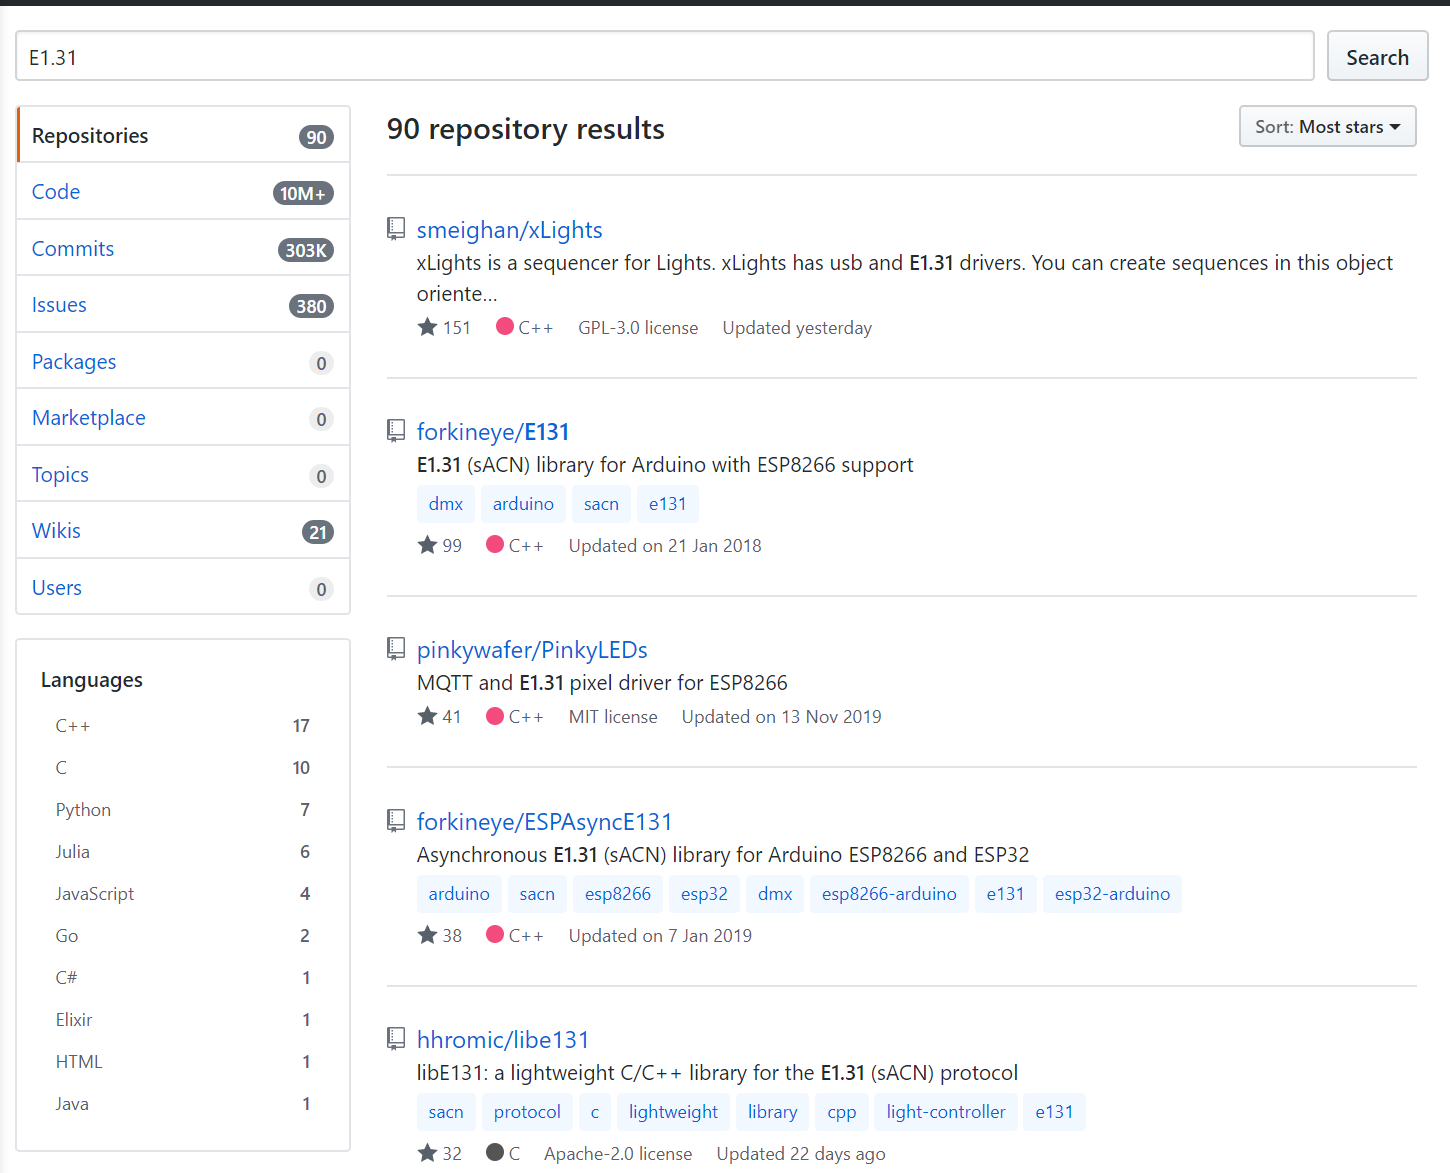
\includegraphics[width=\textwidth]{E131-Repo-Search}
	\caption{A search of repositories on github with the search term "E1.31" as of Jan 2020}
\end{figure}

\section{Requirement specification}
Requirements specification. Capturing the properties the software solution must
have in the form of requirements specification. You
may wish to specify different types of requirements and
given them priorities if applicable.

The project was split into the following list of primary and secondary functional requirements\\
\begin{list}{}{Primary}
	\item Allow sending and receiving DMX data over sACN.
	\item Support the sending and receiving of cross universe DMX data through the universe synchronisation feature.
	\item Support universe discovery with adverts for sources and discovery for receivers.
\end{list}
\begin{list}{}{Secondary}
	\item Demonstrate a deployment of the library into a real-world system to show its compliance with the protocol by showing interoperability with other compliant devices.
	\item Provide support for Windows 10 and Fedora Linux systems.
	\item Support multiple IP transmission modes - Unicast, Multicast and Broadcast.
	\item Support multiple IP versions - Ipv4 and Ipv6.
\end{list}

The intended user for this library is a software developer developing applications that utilise the sACN protocol. It isn't designed to be used directly by an end user as it is just a library which needs to be used in code to actually perform any actions. This means it needs to be able to be understood and utilised by someone who is familiar with general software engineering and the main ideas of sACN. This makes technical documentation of the project code such as comments, API explanations and examples a vital part of the project as otherwise developers won't want or be-able to use the library.\\	

\section{Software Engineering Process}
Software engineering process. The development approach taken and justification for its adoption.

A waterfall based process model was used for the development of the program. In the waterfall method there are several distinct phases of the project as shown in figure: \ref{waterfall-diag} which follow on from each other with loops back possible if a problem is found at a later stage. This development approach was chosen as it has a very clear structure which allows easy to manage distinct milestones so progress through the project can be more easily tracked. This process method has a number of disadvantages as-well with the main one being the inflexibility - if something major needed to change it would be difficult to adapt the project.  As this project is based on a clearly defined specification provided by the protocol specification and the domains were  clearly defined at the start it means that this inflexibility isn't a major issue and so therefore choosing the waterfall method for its advantages makes sense. 

\begin{figure}
\label{waterfall-diag}
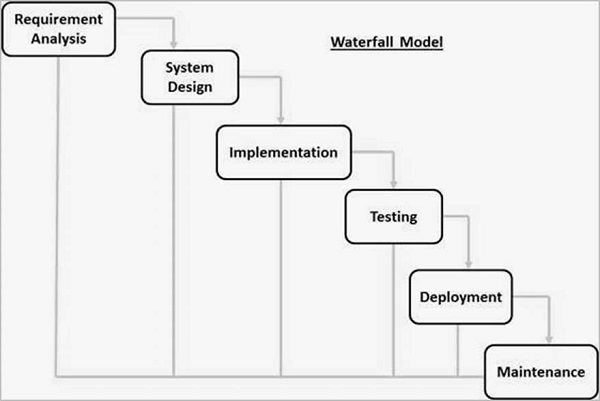
\includegraphics[width=\textwidth]{sdlc_waterfall_model.jpg}
\caption{A diagram showing the waterfall development process, [\cite{waterfall-diagram}]}
\end{figure}

\paragraph*{}
The waterfall model can be clearly seen throughout the development of the program. The first phase of 'requirement analysis' is the protocol specification itself as it clearly lays out the goals of the protocol and what it is required to do. On top of this there is the project goals which were defined around the protocol specifically for how much of the protocol this specification should implement for example universe-synchronisation, IPv4/IPv6 support, Unix/Windows support etc. When take together this gives a clear list of requirements as so allows moving onto the 'system design' phase.

\paragraph*{}
The system design phase is where the requirements are turned into a technical plan for how they will be implemented. Most of this comes from the protocol specification itself as it describes how each bit of a compliant implementation should behave and so therefore the design can be based of this. This combined with the existing base incomplete implementation that was used meant that the general system design was built around this. In general the system was designed around there being distinct receivers and senders with all communication being one-way with no expected replies. This meant that the two different sides could be developed in relative isolation as all their communication must be done in a way that is compliant with the protocol which provides the interface between them.

\subsection{Implementation, Testing and Deployment Phases}
As most of the design is already provided in the form of the protocol specifications and the requirement to make the project in rust it means that the project is mainly focused on the Implementation, Testing and Deployment phases. The implementation phase is one of the biggest in this project and represents the actual creation of the code as discussed in more detail in the Implementation section. As part of the engineering process there was an amount of looping between the implementation and testing phases. This was done as each part of the code was implemented (for example adding universe synchronisation) which was then tested by creating some initial tests to check that the design for that section has been implemented correctly. Then the implementation phase was revisited to either fix a discovered bug or to implement the next section. This looping is similar to the way that a test-driven-development methodology might work however the waterfall methodology described here is distinct as the implementation is written before the tests.\\

The implementation is known to be complete when all the functionality specified in the design has been implemented. In this project this is represented by data sending, universe sync and universe discovery all being implemented on both the sender and receiver. At this point the project moves into the testing phase. The focus now becomes on verifying that the implementation is correct with respect to the design (compliant) using a holistic view with all parts put together as-well as ensuring the documentation matches the actual behaviour. During this stage it is possible that bugs or areas where the implementation isn't compliant with the protocol specification may be discovered. In this case the focus will move briefly back to the implementation stage to fix the problems before progressing back through to the testing phase. It is possible at this phase that a design problem is encountered, for example if it was found that the structure of the program didn't support a functional or non-functional requirement. If this happens then at that point the engineering focus would move back to the design stage and as per the waterfall model the focus would then continue through the process of the implementation and testing phases. The testing phase is signalled as complete when there is sufficient tests that verify that all functional and non-functional requirements have been met. What counts as sufficient is discussed in more detail in the testing section.\\

The next phase if the deployment phase, within the project this is where the finished and tested code is given to users to use. In this project this is shown by the real-world and acceptance tests. These tests fall across the boundary of the testing and deployment phases as they both verify the system works but also show that it is sufficiently mature that it can be used by an intended end user. For this project the intended end user is a software developer creating a program which allows usage of the E131 protocol. Having an actual developer use the library is beyond the scope of the project however the demo sender and receivers act as an example of a possible deployment. Since this example is then demoed by interacting with a real-system and this is shown to someone who actually works in the field it shows that the project has reached the stage of being deployed. As part of this stage it also includes the packaging of the project so that it can be used by developers including the finalisation of documentation and a list of dependencies, once this is complete and the demo programs have been packaged the deployment stage is complete. This is the point at which the scope of the project ends as the final 'deployment' is marked by the final submission.\\

The final stage is the maintenance stage, this falls out with the scope of this limited time-period project however in a real-world project this represents the process of users reporting bugs, problems, feedback and developers looping back to one of the various stages such as design, implementation or testing to verify the problem and implement a fix. While not part of the project directly it is hoped that the library will be able to be contributed back to the community e.g. through the rust cargo repository and GitHub and by doing so the maintenance stage can begin. \\

\subsection{Reflection on Methodology Used}
The approach fit the project well as it made it clear which stages the project was focused on (implementation, testing, deployment) with the previous stages (analysis, design) clearly shown by the protocol specification. The methodology did require increased up-front work as implementation could not begin until the analysis and design states were complete. This up-front work came in the form of the initial documentation for the project such as the DOER list of objectives and as this is required anyway this isn't a problem for this project. The methodology also meant that there was the risk that too long could be spent on one stage which delays further stages and therefore the entire project doesn't reach the deployment stage by the fixed deadline. This meant that a time-line had to be created early on to mark when various parts of the project would be complete so that progress could be tracked. This was attached as part of the project in the 'Objectives with times.txt' file and its creation and modifications are shown by the git-version control which shows how it changed. This was later superseded by minute notes at weekly meetings where the project and its progress were discussed. Taken together these show how the project has developed and how the requirements have been changed from those originally proposed due to time-constraints. \\

A high level view of the development of the project over time is shown in Figure \ref{project_dev_timeline}. This shows that the waterfall methodology was followed starting with the deployed existing library which is moved into the requirement analysis stage as new requirements are set as discussed in the requirements section. The requirements are then turned into a design using some of the structure provided by the existing base implementation and a set of milestones created. As discussed above the project then enters its main stages of implementation and testing which loop around as sections of the program are created, tested and debugged. It can be seen that at on the 12th of January the project had to loop back 2 steps to the design stage and this was due to the non-threaded structure of the program being insufficient to allow the periodic universe discovery adverts and so the design had to be changed to a threaded structure to allow this. The implementation of this new design and testing was then performed as part of the next 2 steps as per the waterfall model. This was then followed by a stage of further testing indicating the start of the test phase. This phase also included instances of steps back being required such as the bug found on March 7th which required implementing a new OS specific socket handling mechanism to fix. The testing phase then continued up until the code was ready to be demoed in the real-world environment which marks the transition from the testing phase into the documentation phase. The documentation phase then continued right up until the final deployment marked by the final submission.\\

\begin{figure}[H]
\label{project_dev_timeline}
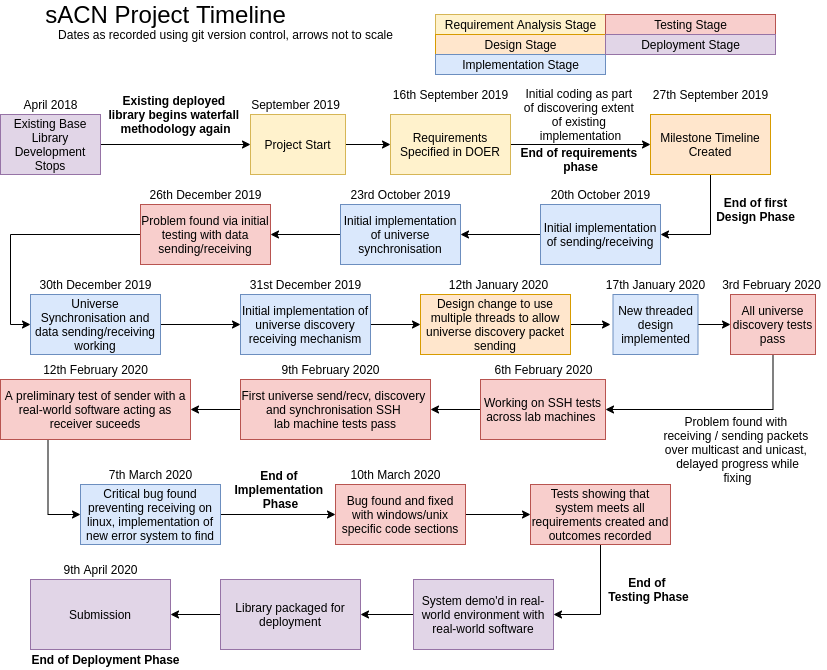
\includegraphics[width=\textwidth]{CS4099-dev-timeline}
\caption{The development of the project over time with the water-fall methodology stages marked}
\end{figure}


\section{Tools \& Technologies}
\subsection{Language: Rust}
Rust \cite{RUST_LANG} is a compiled memory safe language with no garbage collector. It is extremely fast with near C/C++ like performance \cite{RUST_C_COMPARISON} but with a much stricter compiler that guarantees memory safety. As Rust has no runtime due to no garbage collector it is applicable to high performance applications making it an ideal language for an ANSI E1.31-2018 sACN device which are often utilised in environments such as concerts where real-time performance with minimal latency is vital to keeping lighting devices in sync with sound.

\subsubsection{Error handling: Error-chain}
The base implementation provided its own error system based on an Enum with various different types. This had a number of problems, the biggest two being that it didn't allow errors to be encapsulated within each-other to provide a back-trace and it wasn't compatible with errors from rust libraries such as Io and Net. Since this error system was created for the initial implementation there has been significant changes within rust and the way that errors are handled. For example the 'try!' \cite{RUST_TRY} macro which used to return if the item produced an error type has since been depreciated, replaced with the ? operator and try made into a reserved word.\\

Theses issues meant that the existing error implementation was no longer suitable and it didn't make sense to continue trying to use multiple errors systems (rust Io/Net, old system, new errors added by new features). Therefore the entire error system was replaced using the Error-Chain library \cite{ERROR_CHAIN}. This library which is frequently used throughout the rust eco-sphere and allows combining all the error systems into one system with rust errors automatically converted as needed. It also allows errors to encapsulated other errors which allows chaining of errors together to produce much more informative back-traces. As part of this update of the error system all usages of the depreciated 'try!' macro were removed and replaced with the new '?' operator in combination with the error-chain 'bail!' macro. A number of new errors were also added to more descriptively describe possible errors within the library as listed in the 'error.rs' file such as 'ExceededUniverseCapacity' and 'DmxMergeError'. \\

Programs which utilise the library are not required to continue using error-chain within their code and can use their own error systems however for the 'demo\_src' and 'demo\_rcv' programs the decision was made that continuing to use error-chain made sense due to the advantages it provides as described above.

\subsubsection{Networking: Net2 / Socket2}
\subsection{Dependency Management: Cargo}
Within rust libraries/packages are referred to as crates and the management of dependencies is handled by Cargo. This system allows fetching of dependencies as required during the build stage and includes automatic handling of sub-dependencies etc. In addition to this the Cargo system provides many commands related to testing, compiling, documenting and creating rust applications.

\subsubsection{Run}
The cargo run command allows checking of the rust code for compile time errors, fetching of dependencies, compiling/linking of the produced rust binary and finally running the produced binary all within one command. This greatly simplified development as there were no Makefiles or similar to manually manage and the code can easily be moved to a new system for development/testing as required libraries are fetched automatically.

\subsubsection{Docs}
As discussed the targeted end user of the library is a software developer. This makes good comprehensive documentation vital so that developers know what each part of the code does and as this project is expected to eventually be released open-source having good documentation allows new library developers to come in and maintain/expand the code base.\\

Documentation within the project is done using the rustdoc system which is included as part of the rust/cargo development package. This library is very similar to those found in other languages such as Javadoc for Java which work by having documentation embedded within the code which is then transformed into a HTML web-page to provide the documentation for the crate. As it is directly embedded into the code this makes it less likely that it will fall behind as the documentation and code are close together and a developer can change both simultaneously without having to work across multiple different documents. As this is part of the Cargo system it allows the library to packaged up along with its generated documentation automatically so that when it is distributed onto the cargo repository the documentation can be readily accessed alongside.

\subsubsection{Test}
One of the verification methods used with the library is unit tests, these are small self contained tests which can quickly run to verify that a small part of the program behaves as expected. Rust comes with a built-in form of unit testing through usage of the cargo test command. This automatically finds all tests within the code as designated by the test annotation and runs them producing a list of which tests passed and failed. This also includes other tests such as examples in the documentation which helps to prevent problems where examples are forgotten about and as the development progresses become depreciated or broken. Cargo test was therefore an important part of the project during development and remains an important part once the code is in the maintenance phase.

\subsection{Debug Tools: Wireshark}
As a network protocol sACN packets can be inspected on the network and the main tool used for this was Wireshark \cite{WIRESHARK}. This was a crucial debugging tool as it allowed checking that packets were formatted and contained the data that was expected. It was also used to trace a number of bugs related to sending/receiving as it can be used to ensure that packets are actually reaching the destination or if not find where they are lost.  To allow working with sACN specifically wireshark has built-in support for the protocol as-well as displaying the internal DMX payload.

\subsection{Version Control: Git, Gitlab, Github}
Like most modern software engineering projects a version control system was utilised. Even though there is only a single developer and so the collaboration tools were unused during the duration of the project version control still provides significant advantages related to being able to roll-back versions of code if a change must be reversed. This is particularly useful during the final stages of the project where bugs found in testing can be traced to where they were created by testing earlier versions of the code. As-well as the local git repository the code was also pushed onto separate private github and gitlab repositories. This allows development to continue anywhere that can access github and the repository as well as providing two separate backups of the project with one within the school gitlab and one on a private github. The gitlab repository was also useful as it allowed the project supervisor to monitor progress and inspect the project as required.

\subsection{Test Coverage Tool}
The grcov \cite{GRCOV} tool was used to show code test coverage of the library. This tool was created by mozilla and is made specifically for usage with Rust programs. The output of the code coverage is a webpage which contains details of the lines and functions covered for each part of the library, this is then used to find functionality which has been missed in testing. 

\subsection{Compliance Testing Tools: sACN View}
sACNView \cite{SACN_VIEW} is a simple tool which allows sending and receiving with the sACN protocol. It is used as part of the compliance testing of this library as it acts as a real-world deployed version of the protocol which can be tested against. This viewer notably provides support for the universe discovery feature which isn't supported in the other tools used to test compliance so this program is particularly useful for compliance testing with the universe discovery feature.\\

The main page for this tool says it is for the ANSI E1.17 \cite{ANSI_E1.17} protocol (the base ACN protocol) however by this it means the ANSI E1.31 protocol (the sACN part of ACN). The reasoning for this assumption is that at multiple points within the documentation such as \cite{SACN_VIEWER_DOC} it says things such as 'E1.17 (2018)' which must mean E1.31 (a related part of E1.17) as there is no 2018 version of E1.31. The documentation also describes the universe discovery feature which is not part of E1.17 as it is part of E1.31.

\subsection{Real-world Usage Tool: Visualisers: Vision}
When creating a lighting design for an event a common step for a lighting designer is to create a 3D model of the stage and include in it the planned lighting. This allows the designer, clients and project management to see what is being proposed. Once the design is approved the visualiser acts as an accurate simulation of the behaviour of the lighting fixtures and this allows the lighting programmer for the event to create many of the lighting patterns, effects and cues ahead of the actual fixtures being put in place. This is a massive part of any major project as a week spent using a visualiser to create much of what is required for the event in terms of lighting effects is significantly cheaper than a week doing it with the real-fixtures. It also means that the visualisation can be done without being on site which might not be possible if the site is in-use in the time leading upto the event. To allow this programming to be transferred straight onto the real lighting setup most visualisers allow usage of the exact same protocols that are used to control the lights to control the virtual lights. This makes a visualiser an ideal tool with which to test the created library against as a professional visualiser is designed to simulate real-world usage as closely as possible and contains a professional developed/maintained/tested version of sACN. This means that if the library works with the visualiser it shows that it is conformant with an industry implementation which itself is created to be compliant with the protocol and therefore this provides evidence that the library is compliant. From an outside user perspective it also crucially shows that the library can actually be used for its intended purpose. The visualiser that is used for testing this library is Vectorworks Vision \cite{VISION}, this software is professional paid software so for this project the St Andrews Students Association's copy of the software + license was used. Permission for this was granted through communication with the current director of events and services as-well as building management. Vision does offer a free-trial version but this has limited features so by using the full-version it helps better show compliance. \\

The project extends it thanks to the St Andrews Students Association, particularly the director of events and services (Mika Schmeling) for their permission to use their real-world visualiser setup with this project.

\subsection{Real-world Usage Tool: Lighting Control: Avolites Titan}
The visualiser provides a way to test that the library can send sACN which can be utilised by a real-world system but it doesn't test the other-way around where the library is receiving sACN. To test this a source of sACN was required and this came in the form of a real-world lighting controller. The lighting controller used was an Avolites Titan Mobile \cite{AVO_TITAN_MOBILE}. This controller is part of a family of Avolites lighting controllers which are used across the world to control lighting systems with sizes ranging from small few light setups upto huge world-tours. This controller is another professional example of a product which claims compliance with sACN and through its extensive usage by professionals in a variety of systems has show that it is conformant with many systems using the sACN protocol. By testing the library receiver against this lighting controller it therefore adds evidence that it is compliant with the protocol and can actually be used for its intended purpose. This controller was available for the project as I already own it for use as part of my work in the lighting industry outside of university. 

\section{Ethics}
This project has no ethical considerations that require notification in this section.

\section{Design}
Design
Indicating the structure of the system, with particular
focus on main ideas of the design, unusual design
features, etc.

\subsection{Expected System Usage/Layout}
\begin{figure}
\label{Expected_usage}
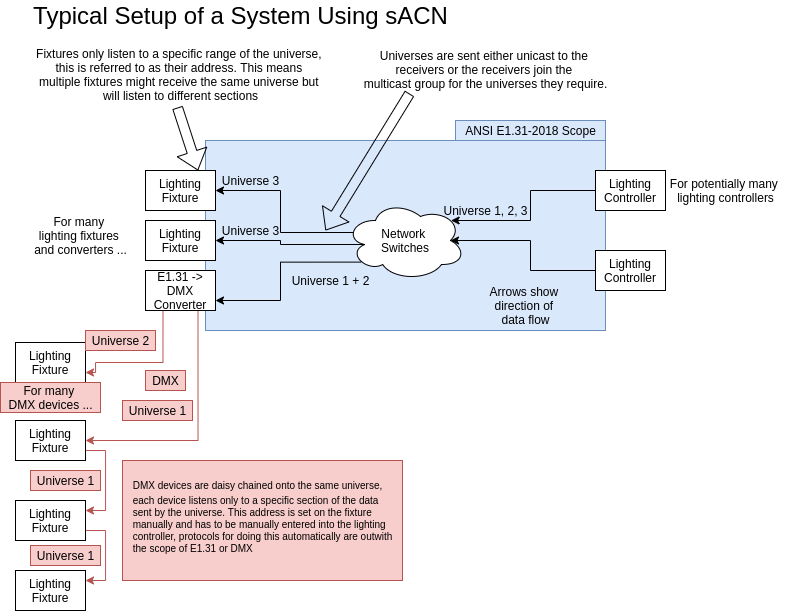
\includegraphics[width=\textwidth]{CS4099-Expected-Usage.png}
\caption{A diagram showing a usage scenario for a system which utilises sACN}
\end{figure}

Figure \ref{Expected_usage} shows a layout of a typical network in which sACN may be deployed. It shows that there are expected to be many sources of sACN in the form of lighting controllers and many receivers in the form of lighting fixtures and E1.31 to DMX converters. It also shows that the senders may send onto the same or separate universes as each other. Receivers can receive one or multiple different universes and multiple receivers can receive the same universes. Within these universes individual devices all have their own 'addresses' which refer to which section of the universe they are listening to as-well as 'modes' which refer to how many 'channels' (Bytes) are used and what each channel controls on the fixture. This within universe addressing as-well as protocols for assigning and communicating addresses that fixtures should use is outwith the scope of ANSI E1.31-2018. The protocol is focused on the section shown in blue which contains the sending of data from sources such as lighting controllers onto receivers such as the lighting fixtures.\\

\subsection{Packet structure}
All sACN packets are based on the standard ACN header as shown in Figure \ref{ACN_HEADER}. By using the general ACN header it allows other ACN protocols to be used on the network alongside sACN without conflicts. To designate the rest of the packet as an sACN packet the vector field is set either to VECTOR\_ROOT\_E131\_DATA to indicate that the packet is a E1.31 data packet or VECTOR\_ROOT\_E131\_EXTENDED (note these are defined constant numbers not strings) to indicate that the packet is either a synchronisation or discovery packet. The rest of the data packet is then structures as specified in Figure \ref{ACN_DATA_STRUCTURE}. For the universe synchronisation and discovery packets the next part of the structure starts the same as shown in Figure \ref{ACN_EXTENDED_START} with the vector field deciding if the rest of the packet follows a synchronisation or discovery packet structure. The synchronisation structure after this is fairly short as shown in Figure \ref{ACN_REST_SYNC_PACKET}. The discovery structure is longer as it may include a list of upto 512 universes and is show in Figure \ref{ACN_REST_DISCOVERY_PACKET}.

\begin{figure}[H]
\label{ACN_HEADER}
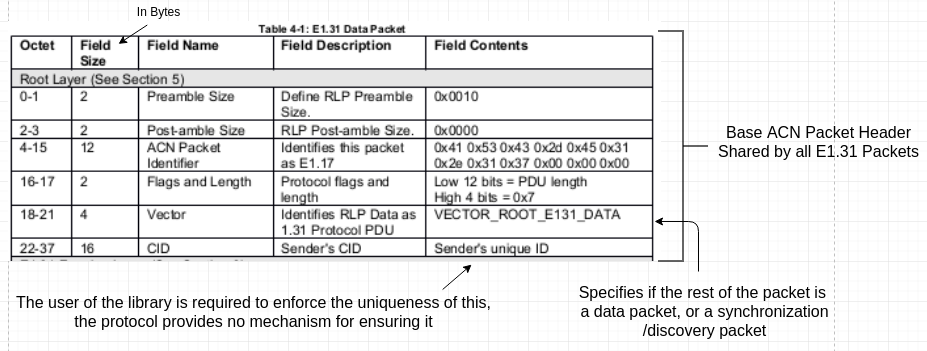
\includegraphics[width=\textwidth]{Acn_header}
\caption{The layout of the standard ACN header used for all sACN packets}
\end{figure}

\begin{figure}[H]
\label{ACN_DATA_STRUCTURE}
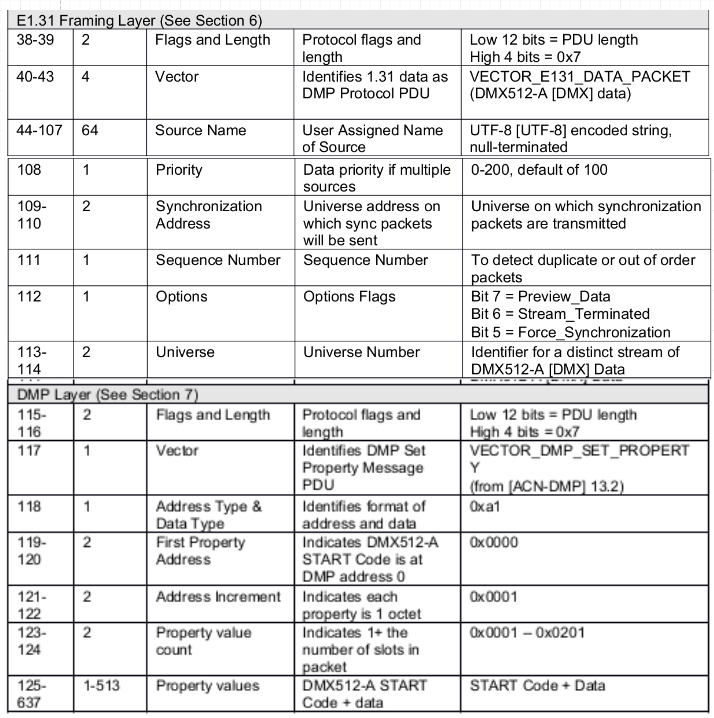
\includegraphics[width=\textwidth]{acn_data_structure}
\caption{The structure of the rest of the sACN data packet}
\end{figure}

\begin{figure}[H]
\label{ACN_EXTENDED_START}
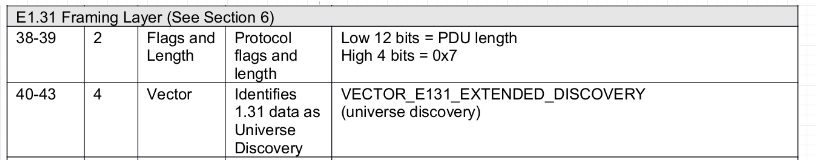
\includegraphics[width=\textwidth]{Acn_extended_framing_structure_sync_discovery}
\caption{The structure of the next part of the sACN universe synchronisation and discovery packet}
\end{figure}

\begin{figure}[H]
\label{ACN_REST_SYNC_PACKET}
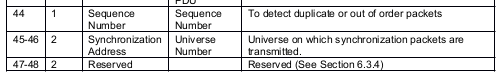
\includegraphics[width=\textwidth]{acn_sync_packet_specific_structure}
\caption{The structure of the rest of the sACN universe synchronisation packet}
\end{figure}

\begin{figure}[H]
\label{ACN_REST_DISCOVERY_PACKET}
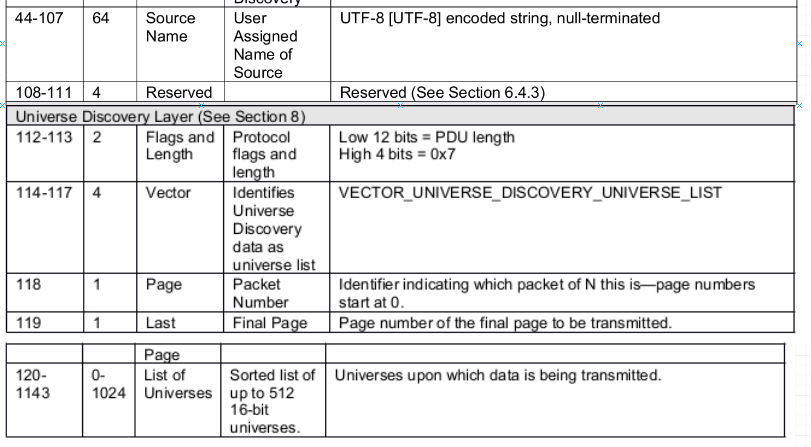
\includegraphics[width=\textwidth]{acn_discovery_packet_specific_structure}
\caption{The structure of the rest of the sACN universe discovery packet}
\end{figure}

\subsubsection{Universe Discovery}
The universe discovery mechanism sends discovery adverts on the 

-- Periodically send universe discovery packets

\subsubsection{Universe Synchronisation}
The universe synchronisation mechanism allows multiple universes of data to be acted upon almost simultaneously. The mechanism for how this works on the receiver side is shown in the include 'Sync-Mechanism.pdf' file as it doesn't fit into the report format in a clear way (splits across pages).

\subsection{Network Layers / Transport Modes}
sACN falls within the application layer of the 5-layer network stack as shown in Figure \ref{NET_STACK}. This is because it sits on top of UDP (layer 4) and IP(layer 3). As UDP is used as the underlying transport protocol it means that there is no guaranteed delivery of packets. The protocol itself also doesn't provide this which means that data send by a source may not reach a receiver and there is no way for the source to know within the protocol scope. This loss of guarantee comes with the advantage that there is less packet overhead and no hand-shake is required meaning data can be sent immediately. The use of UDP also avoids many of the problems associated with session transport protocols like TCP such as lost packets significantly reducing throughput due to the congestion control mechanism. Theses trade-offs fit the expected usage of the sACN protocol as they minimise latency which is vital in a real-time event/lighting system. \\

\begin{figure}[H]
\label{NET_STACK}
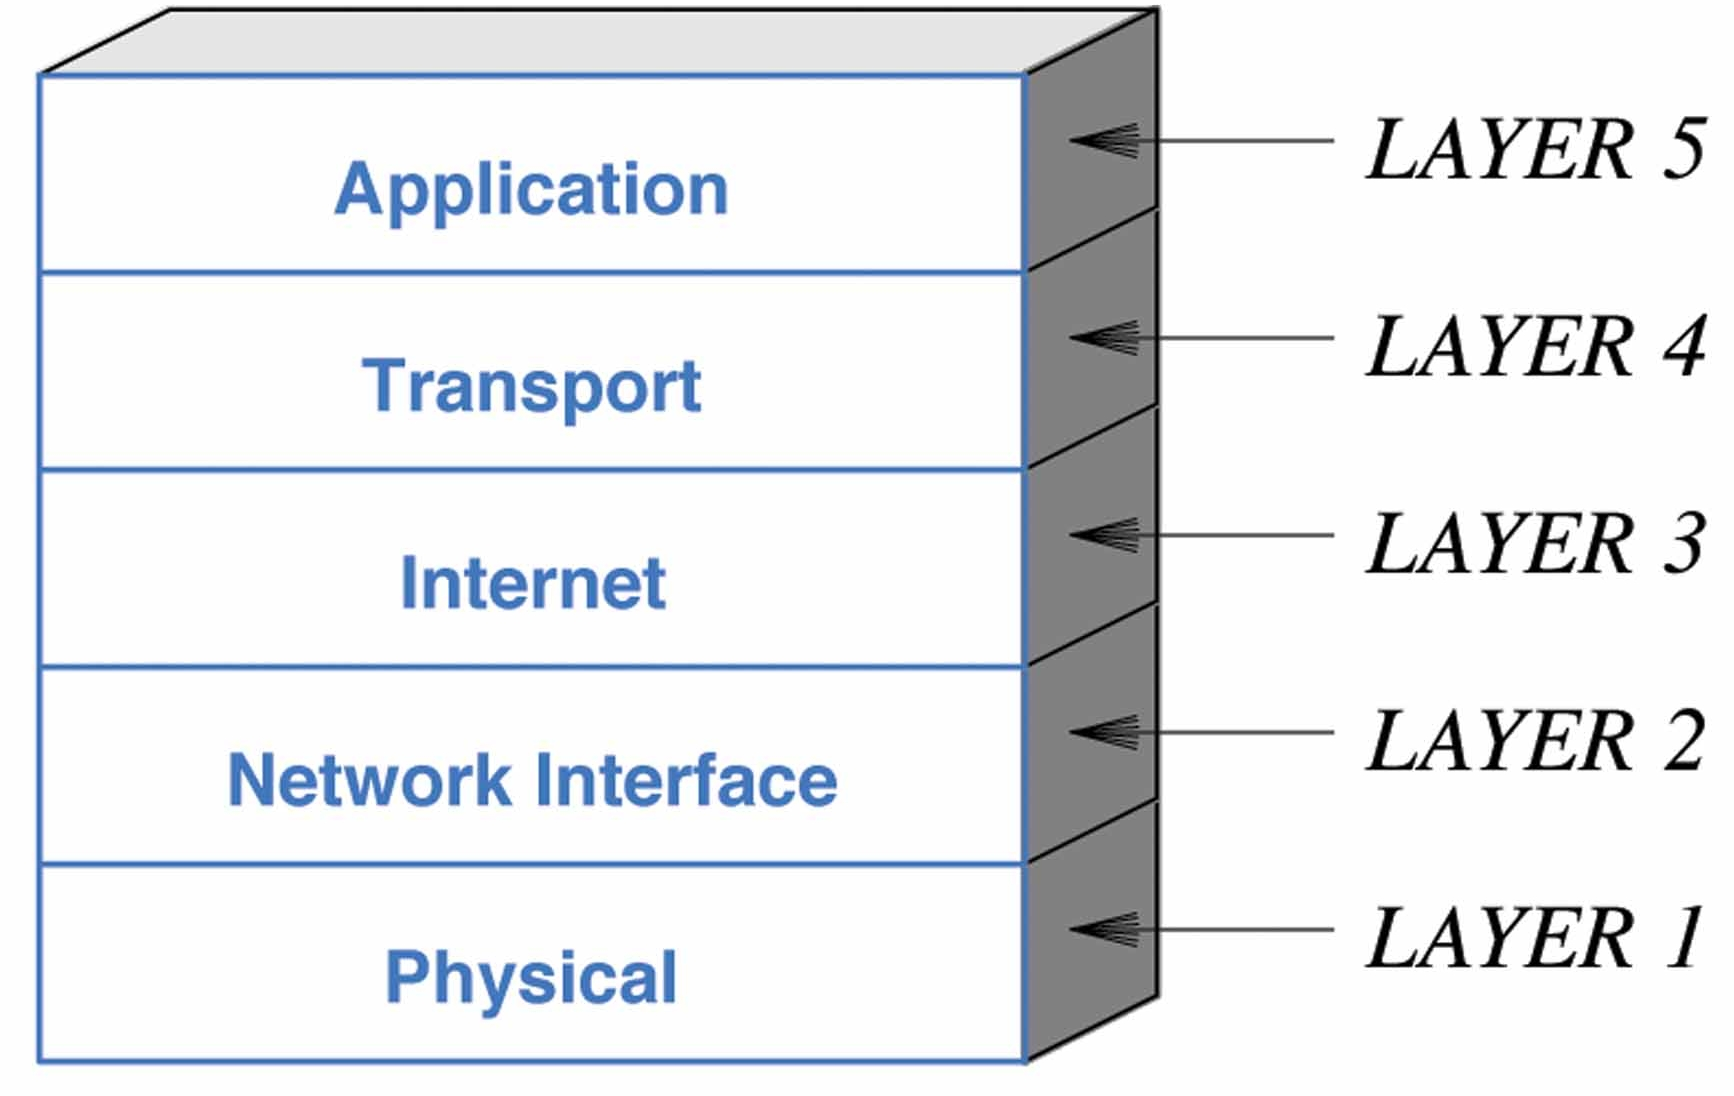
\includegraphics[width=\textwidth]{net_stack}
\caption{Image showing the 5 network layers}
\end{figure}

The usage of UDP additionally means that packets can be delivered in any order, this can cause random jumps in data on the protocol which is noted within the specification to be problematic if this is used with a moving head lighting fixture as it effects the predictive algorithms used (ANSI E1.31-2018 Section 6.7.2). To reduce this happening the protocol uses sequence numbers to allow out of order packets to be discarded. It is important to note that because a packet might have been lost the protocol doesn't attempt to wait for packets which haven't be received yet instead always acting on the most recent data (with regards to sequence number) and discarding any old data received. This keeps the latency of the system low and prevents slightly out of order packets causing unexpected jumps back and forth in the data. As the sequence number field is only 1 byte in length it is expected to wrap around frequently, therefore the sequence numbering mechanism accounts for this by looking at the difference between the last and current sequence numbers as oppose to the numbers themselves directly. This combined with using a reject range for the difference of (-20, 0] with other values accepted allows for the sequence number to wrap around and for the system to quickly (within 20 sequentially numbered packets) start accepting packets again - once again minimising latency. 

The protocol is specified for usage over IP however it doesn't have any inherent requirements for this meaning that in future it could be used over another network protocol with a suitable adaptation. This makes the protocol more future proof and more widely applicable to different applications which might be non-IP. In its current 2018 state however the protocol only specifies operation over IPv4 and IPv6 using 3 different communication modes. The first mode is unicast, this is where a source sends data directly to the receivers IP and this means that any data sent by a source must individually be sent to all receivers for them to see it. The next mode is broadcast, this is where the destination IP is set to a special broadcast IP which causes all receivers to see the data. This mode means that a sender doesn't have to individually send to each receiver but does mean that there is the potential to flood the network with these broadcast packets with all receivers getting packets even if they didn't want them.\\

The final IP communication mode utilised by the protocol is IP Multicast. This is the default mode used and works by receivers joining ip multicast groups which senders then send to with only the receivers that joined the relevant multicast group seeing the send packets. This minimises the packets sent with only registered interested receivers seeing packets. Within the sACN protocol each universe utilises a different multicast address and therefore each receiver and sender can use a specific address to receive from / send to a specific universe. This assignment of addresses to universes is described below.\\

\subsubsection{Multicast Address Assignment}
For a sACN universe IPv4 multicast address the first 2 bytes are always 239 and 255 respectively. The 3rd byte is the upper, most significant byte of the universe (when the universe is expressed as a 2 byte unsigned number) and the 4th byte is the least significant byte. This is shown by Figure \ref{IPV4_MULTICAST_MAPPING}.

\begin{figure}[H]
\label{IPV4_MULTICAST_MAPPING}
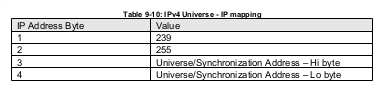
\includegraphics[width=\textwidth]{Ipv4MulticastMapping}
\caption{The mapping used from a universe to an Ipv4 address used for multicast with sACN}
\end{figure}

The Ipv6 mapping is similar with the least significant 16 bits used, Figure: \ref{IPV6_MULTICAST_MAPPING}.

\begin{figure}[H]
\label{IPV6_MULTICAST_MAPPING}
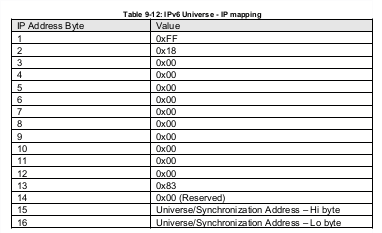
\includegraphics[width=\textwidth]{Ipv6MulticastMapping}
\caption{The mapping used from a universe to an Ipv6 address used for multicast with sACN}
\end{figure}

As specified in the internet engineering task force (IETF) RFC 5771 \cite{IETF_RFC_5771} all of the Ipv4 multicast address fall within the 'Administratively Scoped Block' as specified in IETF RFC 2365 \cite{IETF_RFC_2365}. This then clarifies that the sACN multicast address fall within the IPv4 Local Scope range (6.1). These multicast addresses are reserved for usage dependent on the specific local network within which they are deployed. This limits the sACN usage to a local dedicated network and not for use on a wide area network (WAN) for as the public internet. As discussed previously this fits with the other design decisions made which based the protocol around usage on a private, isolated dedicated network.\\

The IPv6 multicast address assignment starts with 0xFF in the first byte, this indicates that the address is a multicast address. This is then followed by 0x18 which can be broken down as per section 2.7 of \cite{IETF_RFC_4291} into a flag value of 1 and a scop value of 8. This flag value mean that this is a transient address which indicates that it isn't statically assigned by the IETF and may change in future. The scope value of 8 indicates organisation-local scope which has a similar reasoning as the local-scope used for IPv4 meaning that this address is only valid within a specific environment / group of networks. Therefore the sACN protocol is not aimed at usage on a WAN regardless of Ipv4 or Ipv6. 

\section{Implementation}
Implementation
How the implementation was done and tested, with particular focus on important / novel algorithms and/or data structures, unusual implementation decisions, novel user interface features, etc.

-- Limitations, only does IPv6 or IPv4 at one time.


\subsection{SacnReceiver}
The project was based around creating a library that is high-level enough that a user can easily use it for its primary functionality. This meant providing a clear set of public facing functions/methods which don't rely on the user understanding all aspects of the protocol and instead just the bits they are interested in. For example the SacnReceiver.recv(timeout) method which takes just a timeout (using None to indicate no timeout) and returns DMX data. This completely abstracts away many aspects of the protocol from a user who most of the time will want to just get data and perform actions with it. For example this function abstracts the concept of universe synchronisation with data only retuned when it is ready to be acted upon without users having to know when they can use the data. This also abstracts away having to handle universe discovery packets, if a universe discovery packet is received then by default it is handled silently and added to the receivers list of discovered sources. This allows the user the flexibility to inspect the list of discovered sources if required but otherwise they can be ignored. This decision to not explicitly announce the discovered universes was made with the observation that a receiver spends most of its time receiving and processing data rather than listing discovered sources - especially as a source doesn't have to be 'discovered' to allow receiving on. This design decision comes with a few trade-offs, first it means that to discover sources a receiver must first attempt to receive data even if it doesn't act on any received data. This leads to a pattern of attempting to receive data with a short timeout and then inspecting the list of discovered sources. This is slightly more work for a library user trying to discover sources but allows the flexibility for the user to choose how they want to handle data received in this time (throw out or handle). The library does allow setting a flag on the receiver to change this behaviour, if the 'announce\_source\_discovery' flag is set to true (default is false) then on completely discovering a source the method will return a SourceDiscovered error. This still means any data received will need to be handled by the user but means that if no data is received it prevents the method having to wait for the entire timeout if a source is discovered. By having this off by default it keeps the method functionality simple for the expected majority of the receivers time when it is just receiving data but allowing the flexibility for use-cases that require knowing whenever a source is discovered. An error was used as oppose to a special return value for a similar reason - to keep it simple for the major use case. This is similar to how the underlying socket will return a WouldBlock or TimedOut error if it doesn't receive within the given timeout, this isn't explicitly an error that means the program has to stop operation but it is something that the user should handle. Since errors are handled as part of the type system adding an error also doesn't add significant performance overhead. \\

-- ANSI E1.31-2018 Section 8.5 specifies that the list of universes in a universe discovery packet must be sorted numerically but doesn't specify if this should be in accending or decending order. The implementation assumes accending order however this exists as a potential source of compatibility problems between implementations due to this being unclear in the specification.


\subsection{SacnSource}
Unlike the receiver on the sender side universe synchronisation has to be handled explicitly. Firstly when data is sent there is an optional synchronisation universe argument. The rust built in Option type makes this simple to ignore if not required as this can be set to None to indicate no synchronisation. When data is sent with synchronisation it won't be acted upon until a synchronisation packet is send using the 'send\_sync\_packet' initially the sender would automatically send this sync packet after the data was sent however this was removed and an explicitly split up method used instead. While slightly more involved this provides greatly increased flexibility because with the other method there was no way for a source to send data and either synchronise it later or to allow another source to generate synchronisation packet. While not a hard requirement it is advised in the standard (ANSI-E1.31-2018 Appendix B.1) that there is a small delay between sending data and sending the synchronisation packet to allow receivers time to process the data. This isn't enforced by the library as what counts as a 'small' delay will depend on the system and so this is left up to the user to decide. Similarly as specified in ANSI E1.31-2018 Section 6.6.1 the send method shouldn't be called at a higher refresh rate than specified in DMX (ANSI E1.11) unless there are no E1.31-DMX converts on the network. Since this is also something which is system dependent and the library cannot know on its own this is also left to the user.\\

The send method also exposes the way that the information is sent on the network through the 'dst\_ip' this argument allows a sender to send information using unicast directly to a source (or broadcast by providing the broadcast IP) but also allows usage of multicast (as described in design) by providing the None argument. \\

The sender is based on a multi-threaded model with an internal source protected by a lock encapsulated within the SacnSource that users interact with. The reason for this was to allow abstracting the task of sending periodic universe discovery packets away from the user. Instead on creation the SacnSource spawns a thread which will send universe discovery packets at the 10s interval defined in ANSI E1.31-2018 Appendix A. This leads to the requirement for a user to register a universe before they can send data on that universe allowing it to be reflected in the discovery packets. By abstracting this behaviour away it makes it easier for the users to create a compliant source as the correct sending interval and formatting (including splitting into multiple pages) is handled for them. In some situations it might be required that universe discovery isn't used, for example if there are devices which implement ANSI E1.31-2009 which was created before universe discovery and which don't correctly discard packets with the wrong vector. To allow compatibility with these devices the sender provides the 'is\_sending\_discovery' flag which defaults to true but can be set to false to prevent discovery packets being sent.

\subsection{Std vs Non-Std}
The library is implemented assuming a std environment. This means that the rust std libraries such as the network library are available. This greatly increases the amount that can be done using rust as within the standard library the inbuilt functionality is fairly limited and would require rebuilding many already implemented solutions. This differs from the library that the implementation is based on which allowed running in environments with and without std. The reason to discontinue support for no\_std environments was made as the new parts of the protocol which were being implemented such as universe discovery are significantly easier and provide a better user experience when parts of the standard library such as the threads can be used. \\

\subsection{Drop / Closing}
Unlike many languages the underlying rust socket used for this library does not require being explicitly closed as it automatically cleans up when it is out of scope. This protects against an entire family of errors related to incorrectly closed/not-closed streams. In-line with this the library also cleans the created receiver/sender up automatically through the implementation of the 'Drop' trait. As part of this the implementation decision was made that a source will automatically terminate any universe it is currently sending on (as well as its spawned thread), this is similar to a TCP stream sending FIN packets to close. The receiver will also de-register any universes it is listening on by leaving the multicast groups it has previously joined. \\

During a Drop there is no provided way to pass an error to the user. This is inherent in Drop being called automatically because there is no clear return path for an error nor can the Drop be stopped either-way as it might be called during a panic! or program wrap up. This leads to an implementation decision for how to handle errors with 4 distinct options: panic, notify, prevent, ignore. Panic means that within the drop if there is an error then panic the program with a description of the error. This notifies the user however it also causes the program to be terminated even if it could potentially continue. It also pollutes the error-output and can lead to the original error/problem to be hidden. This makes it unsuitable for this application as a failure to drop won't lead to memory unsafety or otherwise cause significant problems beyond the program scope. Notifying the user refers to using a functionality such as logging, printing to standard-out or some other mechanism. Printing to stdout is avoided as this might pollute an applications output by displaying errors to the user which a developer using the library might want to avoid. Logging is a possible option which adds further complexity to the library as-well as another requirement for a logging library. Preventing the possibility of the error is the ideal solution however in this case as IO is required this cannot be guaranteed if there is a problem with the underlying socket. The final solution is to ignore the error, usually this would be problematic as it doesn't allow the application developer to decide the programs behaviour or to fix the problem but in this case that isn't possible anyway. Ignoring the error also allows as much to be cleaned up as possible unlike panic which would stop cleaning up at the point the error occurs. The actual implementation decision based on this was therefore to ignore the error with the recommendation that logging could be potentially added later.

\section{Testing}
As a software engineering project the testing stage is vitally important and took up a large amount of the total time spent on the project. The key aims of testing are as follows, first to show that the code works as intended. This is primary done through the unit and integration tests. The next part is showing that the code works as expected by the protocol. This is referred to as compliance testing and as creating a library that is compliant with parts of the ANSI E1.31-2018 protocol was the main aim of the project this compliance testing is crucial to showing the success of the project. The final aim of the testing is to show that the library is actually suitable for usage, this comes in the form of acceptance testing where the library is actually utilised for its intended purpose by an end user.\\

These 3 aims show that the project works as intended, that the intended functionality is compliant with the protocol and that the project can actually be used for its functionality by a user. Once the project has successfully passed these 3 categories of tests it is ready to move onto the deployment stage of the software development life cycle.

\subsection{Scope}
Within these testing objectives 3 types of tests were used Normal, Extreme and Exceptional. Normal testing involves situations which are expected by the project such as in this case receiving data from a registered and expected universe.The basic requirement of the project to be successful is for it to pass all normal testing as this shows that the project actually performs the intended functionality. Extreme testing is similar to normal testing but with the situations being on the edge of what is expected/allowed, for example sending a full data packet is an extreme test as it is on the edge of the allowed data packet length. Extreme tests show the bounds of the project and highlight where normal, expected scenarios transition into exceptional scenarios. Exceptional tests are where the project is tested with scenarios and inputs beyond what is allowed. In these cases the program must take some action to handle the scenario, in many cases exceptional input may put the program into an undefined or failing state. This action is undesirable however because it means that there is no way to know exactly what will happen or in some cases to stop the program from crashing. This is especially problematic for this project as it is a library which should be usable by developers within their projects and different usages of the library will need to handle errors in different ways. The project therefore attempts to prevent undefined or crashing behaviour by flagging up exceptional input or scenarios before they cause a crash (called a panic in rust). This flagging is done by methods/functions being able to return a Result type which explicitly encodes the possibility of either an Ok' non error result or an 'Err' error result. The aim of the exceptional tests therefore are to show that even when provided with unexpected scenarios such as those out-with the ranges given by the protocol that the implementation follows predetermined behaviour that allows the user of the library to handle or correct the problem.\\

The testing aims to provide coverage of the entire library including the parts from the existing implementation. This is important because the existing implementation lacked sufficient testing and in multiple cases it was discovered that it had problems including multiple deviations from the protocol specification. One example of this was the 'options' field within the data-packets. The existing implementation took bit 7 to mean the 7th bit which is incorrect as specified in ANSI E1.31-2018 that the 7th bit means the most significant bit and the 0th bit is the least significant. This problem meant that the existing implementation did not correctly assign the option flags leading to malformed packets and this is a problem which was prevented through testing. In this case the problem was verified to be fixed both through unit testing and by utilising wireshark to verify that it was interpreting the option field as expected once the change was made. This highlights why thorough testing is so important as small differences which have a big impact such as this are easy to miss when developing and unlikely to be spotted in a developer 'dry-run'.

\subsection{Testing Mechanisms}
A priority was put on reproducibility and automation when it comes to testing. The reasoning for this is once a framework is set-up it takes approximately the same time to run a test manually once or twice as it does to write the test in a way that it can be run multiple times automatically. This means that there is only a small penalty to setting up a test so that it can run automatically but once it is set-up it can be run frequently allowing confidence that the code continues to work and that any change such as a bug fix for another test hasn't broken something else. Easily reproducible automated tests also provide a significant advantage to a project once it reaches the deployment/maintenance stage as they act as further documentation of the code and a source of examples for new developers to use when learning. These examples are particularly good as they can be run to verify that they still perform as expected which can be used to flag up areas where the documentation and code have diverged.\\

\subsubsection{Unit Testing}
Unit tests focus on a small specific part of the program to test its functionality for example a single method or functionality. The goal of these tests are to be quick to run and show that each individual part of the project work. By having unit tests for each part of the program is allows showing that individually all the bits of the project work. As these are quick to run they are run after each change/bug fix made during the testing stage of development and show that the fix hasn't introduced any issues into already working sections. This sped up the implementation and testing phases by allowing problems to be identified and fixed quickly. These tests are also an important part of the maintenance stage for a similar reason.\\

Unit testing relies on testing each unit to be effective and so therefore as part of testing a code-coverage tool was used. This goes through the code and highlights areas that are missing tests thereby making it easier during testing to identify missed areas. It isn't perfect as it cannot check if every possibility/situation has been tested for every function but acts as a guide to improve testing.\\

As described in the tools section unit tests created using the in-built rust/cargo unit testing framework. In addition to this the code coverage of these unit tests was checked using the grcov tool created by mozilla \cite{GRCOV}. The output of the test coverage is included as a webpage (index.html in the coverage folder) and the library view of the results are shown in \ref{GRCOV_TOP_LEVEL}. The library is focused on as this is the focus of the testing (the other modules are part of the webpage but not shown in the screenshot). The code coverage tool shows that ... 

\begin{figure}[H]
	\label{GRCOV_TOP_LEVEL}
	
\includegraphics[width=\textwidth]{todo.jpg}
	\caption{The library view of the code coverage tool output showing the code coverage of each part of the code}
\end{figure}

\subsubsection{Integration Testing}
Unit testing shows that individual parts of the code works as expected, integration comes as the next step where the parts are tested (integrated) together. This included testing the sender and receiver as full units as well as testing them with each other. This was done using two separate mechanisms. The first utilised the rust testing framework that already exists (as used for the unit tests) by creating multiple threads within a test with each thread representing a sender or receiver. These senders and receivers then connect to the same network using different addresses and generate/receive packets to check the output in a variety of scenarios. This simulates the senders and receivers being independent as they only share data through the protocol with no shared memory (sharing memory between threads can only be done explicitly in rust a normal variable cannot be shared). The only exception to this was the usage of the rust thread message passing system which allowed the sender/receiver threads to wait on each other as appropriate to allow repeatedly creating the desired test scenario. An example of this is shown in figure \ref{UNIT_INTEGRATION_TEST}. This shows how a typical test is set-up . First the constant parameters are defined first. Second the senders or in this case receiver created are created. The sender/receivers are then put into the expected states by using the thread message passing to communicate as certain points are reached in the code which in this case is the receiver being ready to receive. The actions being tested, in this case sending a single universe of data over multicast, are then performed and the outcome is checked against the expected results. These integration tests mimic the real-usage of the system but with the advantage that the states of the sender/receive can be more easily synchronised to test a specific scenario using the thread message passing system. These tests can also be run on a single machine utilising a feature within both Fedora and Windows which allows a single interface to a network to use multiple IP addresses. This is required because the receiver must use the protocol defined ACN port and so different addresses have to be used to provide separation. As the states can be easily synchronised and only a single computer is needed these tests allow a large range of possible scenarios and functionality to be checked without requiring a more complicated (and prone to breakages) set-up. 

\begin{figure}[H]
	\label{UNIT_INTEGRATION_TEST}
	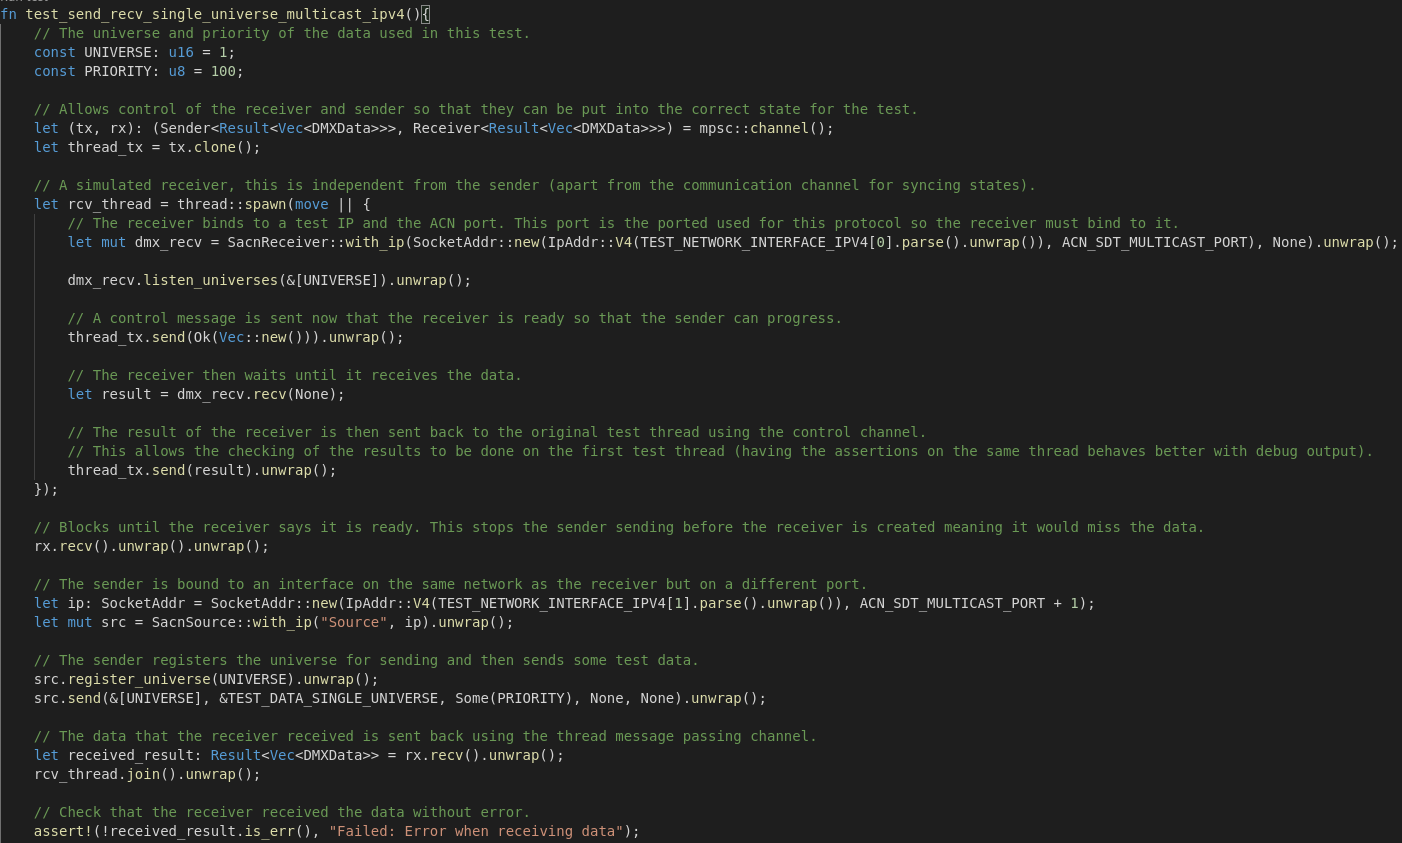
\includegraphics[width=\textwidth]{integration-test-example.png}
	\caption{}
\end{figure}

The threaded integration tests are limited because the protocol is designed to work across multiple machines and the tests only use one machine. This means that to fully test the protocol it also has to be tested in a more representative environment of its actual usage. In-order to allow this 2 small demo programs were created, these programs were also written in rust and represent an example implementation of a sender ('demo\_src') and a receiver ('demo\_rcv') that uses the library. A testing framework was then created as shown in the 'script-testing' folder. This framework works between multiple machines by using SSH to start up the required senders and receivers and then predefined input is provided to both and the output written to a file on a shared file system. Once all the tests are run the output is then compared against the expected output (utilising the diff tool) and if it matches the test is marked as passed (failed otherwise). This allows a way of showing the that the protocol works across a real network setup with multiple machines while still being reproducible without having large amounts of manual input. This test setup can be represented as the abstract and physical layout shown in Figure \ref{INTEGRATION_TEST_SETUP}.

\begin{figure}[H]
	\label{INTEGRATION_TEST_SETUP}
	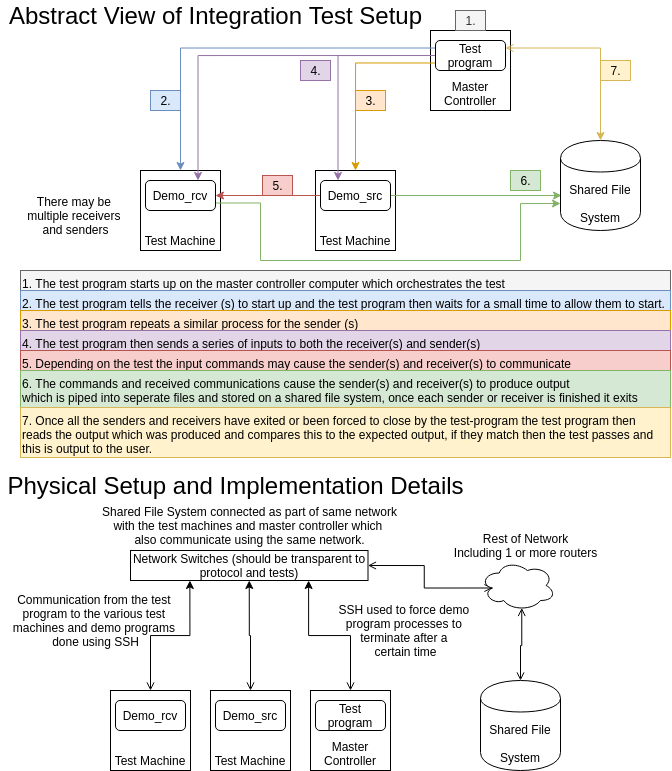
\includegraphics[width=\textwidth]{SH-Project-Intergration-Tests-Abstract-View.png}
	\caption{The abstract setup of the integration tests along with the actual implementation}
\end{figure}

The test-scripts used as-well as the expected output files and given inputs are included in the integration-testing folder. The test\_run script actually runs the test, it starts the receiver and sender and then provides the receiver the commands in the 'rcv' file and the sender the commands in the 'src' file. The output of both sender and receiver are piped into an output file 'xrcv-out.temp' and 'xsrc-out.temp' where 'x' is the test number. The test\_check script then checks the output against the expected output for each test and reports pass/fail. The reason for separate run/check scripts is that it helps to account for the delay in the file-system syncing the output from the test machines so that the master can check it.

\subsubsection{Fuzz Testing}
The integration and unit tests are both focused on checking behaviour of the protocol in specific conditions. What this doesn't check however is the behaviour of the protocol when given a wider variety of inputs. Where this is particularly important is with the packets parsed from the network. It is possible that there may be multiple different protocols operating on a network and so therefore it is possible that the implementation may receive packets from these sources. It is also possible that there may be malfunctioning/malicious sources on the network sending random or scrambled data. This means that the protocol should be able to handle this by flagging up malformed packets without crashing. This is particularly important in this case because this library may be used within an implementation of a show-critical device and so therefore should avoid crashing as much as possible. To test how well the library does in this regard a technique called fuzzing is used. This is where a fuzzing program generates data (based on some initial inputs) which it then feeds to the program being tested and it checks if the program crashes. This fuzzing program does this continuously using a huge variety of possible data while recording how the program handles it each time.\\

For this test the american-fuzzy-lop library \cite{RUST_AFL_FUZZ} was used. This was setup as described at \cite{RUST_AFL_FUZZ_DOC} and run on the Fedora 31 operating system. The fuzz target code used is included in the sacn-parse-fuzz-target subfolder of the Fuzzing folder. This code is extremely basic and just passes the provided fuzzing data straight to the parse function and ignores the result. This therefore doesn't check the error returned or if a specific packet is parsed but it doesn't check that the library parsing mechanism runs without encountering a crash (a rust panic!).\\

To guide the fuzzer to produce data based on sACN expected packets the raw data for a data, synchronisation and discovery packet are used as inputs. These packets are found in the 'fuzz\_in' subfolder of the Fuzzing folder. The packets were generated by performing a wireshark capture of the implementation sender sending these packets and this is included as the "fuzz-test-base-captured-packets.pcapng" file. These captured packets were then transformed into raw data files utilising the wireshark export raw data export feature as described in \cite{WIRESHARK_EXPORT_RAW}.\\

The results of the fuzzer run are shown in figure \ref{FUZZ_RESULTS}. These results show...

\begin{figure}[H]
	\label{FUZZ_RESULTS}
	
\includegraphics[width=\textwidth]{todo}
	\caption{The results of the fuzz testing on the parsing part of the library.}
\end{figure}

\subsubsection{Testing External Interoperability}
The unit and integration tests show that the program works within itself but it is unlikely that within a deployment scenario only a single implementation would be used and so therefore it is also required to show that the library is interoperable with other programs. Since all the programs run the same protocol it is expected that they should all be able to communicate. \\

These tests can highlight problems with the program which are hidden until this point such as gaps in the specification where the library behaviour is implementation defined and may not be compatible with other systems. It can also highlight parts of the system which perform slightly differently than described in the abstract specification due to the introduction of real-world factors such as real-equipment limitations like processing speeds. An example of this might be if the library absolutely relied on universe discovery packets being sent at exactly the interval as defined by the specification. In-real systems network delays as well as varying workloads on the devices might cause packets to be received at slightly variable intervals. Real-world tests therefore help find some of these problems and allow fixes to be made before the program is sent to users.

\paragraph*{Industry Sender - Avolites Titan Setup}
To allow repeatability the show files used for the interoperability tests are included in the Avolites Titan Show Files sub folder in the Interoperability Testing folder. These show files were made for version 11.4 and run on an Avolites Titan Mobile. Within the show file each universe was assigned to an sACN universe with a 1 to 1 mapping and no other network protocols were used as shown in figure \ref{AVO_DMX_LINES}.  In addition to this within the show-file itself 1 channel lighting fixtures called 'dimmers' were used to allow a 1:1 mapping between a fixture in the show-file and a DMX-address. This mapping is shown in figure \ref{AVO_RECV_INTEROP_SETUP} which shows some of the dimmers used (the groups part of the window shows that 8190 dimmers were added to represent each channel in universes 1 - 16). All settings used are included within the save files but in general were left to their defaults.

\begin{figure}[H]
	\label{AVO_DMX_LINES}
	\includegraphics*[width=\textwidth]{avo-dmx-lines.png}
	\caption{The setup of the avolites show file network protocols used for the interoperability testing}
\end{figure}

\begin{figure}[H]
	\label{AVO_RECV_INTEROP_SETUP}
	\includegraphics*[width=\textwidth]{avo-file-dims.png}
	\caption{The setup of the avolites show file used for interoperability testing showing some of the fixtures patched}
\end{figure}

\paragraph*{Industry Receiver - Vectorworks Vision Setup}
The vectorworks vision visualiser uses the vision files "CS4099-TEST.v3s" and "Student-Union-Model.v3s" included within the Test Resources folders of the Sender Interoperability Testing and Acceptance Test folders. Vision was setup using medium graphical quality settings although this should have had no effect on the results. The patch used within each file is included within the file itself as is the positions of each individual fixture. The 'DMX Provider' setting was set to sACN for all tests. The tests were performed on Vectorworks Vision Plus 2019 with a professional license and version 24.0.6.521266.

\paragraph*{Industry Receiver - sACNView Setup}
sACNView was setup using the default settings with the ethernet interface assigned to 192.168.0.6 set as the network interface as shown in figure \ref{SACN_VIEW_INTEROP_SETUP}. Universes 1 - 16 inclusive were listened to for every test even if less than that were used for a specific test. Unicast and multicast were enabled for every universe as shown in figure \ref{SACN_VIEW_UNICAST_MULTICAST_ENABLED}.

\begin{figure}[H]
	\label{SACN_VIEW_INTEROP_SETUP}
	\includegraphics*[width=\textwidth]{sacnViewSettings.png}
	\caption{The setup of sacnView used for the interoperability tests}
\end{figure}

\begin{figure}[H]
	\label{SACN_VIEW_UNICAST_MULTICAST_ENABLED}
	\includegraphics*[width=\textwidth]{sacnViewIPmodes.png}
	\caption{The IP modes enabled in sacnView used for the interoperability tests}
\end{figure}

\paragraph*{Testing receiver implementation}
To show that the sACN receiver implementation is interoperable with a real-world sender the demo receiver program was set-up and run in a network as shown in figure \ref{AVO_SETUP} along with an professional industry source of sACN in the form of the Avolites Titan program as described in the tools section. The tests run and what they demonstrate are detailed in the included "CS4099 - Interoperability Testing.pdf" document. The real-world implementation used doesn't support sending universe synchronisation or universe discovery data so these could not be tested in this step however details of how theses would have been tested are also included in the document.

For some of the tests it was easier to determine if they passed by visualising the received data. In test 5 the sender sends data on 16 different universes with different value ranges per universe. For this test to pass each universe should only contain the values within the range assigned to it as specified in the testing document. To show that this was the case the results were output to a csv file "test-5-out.csv" and then processed using a spreadsheet "test-5-data-processed.xlsx" to produce the graph "test-5-processed-first-value-chart.png" which is included in figure \ref{RCV_INTEROP_TEST_5_GRAPH}. This graph shows that each universe stays within the range expected and therefore that the test passes. As a sanity check of the results this test was also repeated using the sACN-viewer as the receiver and the graph produced in real-time recorded and included as the "Test-5-Receiver-Control-sACN-Viewer.mkv" file.\\

Similar to test 5, tests 3 and 4 also included visualisation elements as part of the check and details of these as-well as further specifics/details of all tests are included within the screenshots/videos within the relevant folders test folders (excluded from report for brevity).\\

\begin{figure}[H]
	\label{AVO_SETUP}
	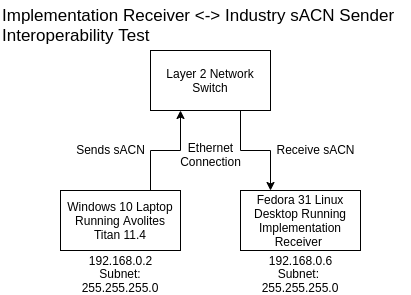
\includegraphics[width=\textwidth]{CS4099-Avo-setup.png}
	\caption{The set-up of the text with the implementation receiver and an industry sACN source}
\end{figure}

\begin{figure}[H]
	\label{RCV_INTEROP_TEST_5_GRAPH}
	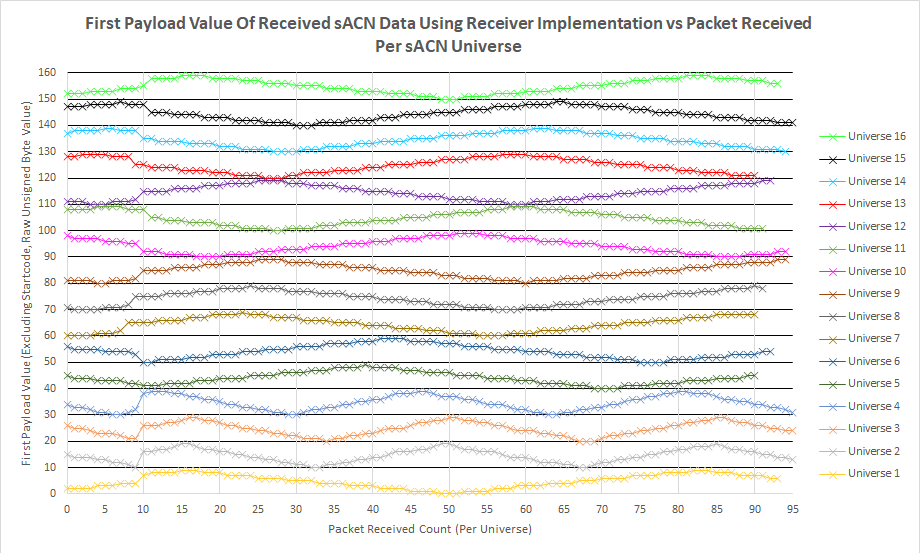
\includegraphics[width=\textwidth]{test-5-processed-first-value-chart}
	\caption{A graph showing the values of each universe per packet received for that universe. This shows the ranges of each universe fit within the expected.}
\end{figure}

\paragraph*{Testing sender implementation}
Similarly to test the sACN sender implementation an external receiver was used. In this case 2 separate receivers were used, the vision visualiser and sACN viewer, as discussed previously. Separate programs were used because neither program was suitable on its own. The visualiser was created by a large company within industry and is used every day by professionals working in the field. This gives a high confidence that it will be compliant with the protocol and so showing interoperability with this is very valuable. It was found however that the visualiser only supports data packets and does not support universe synchronisation or discovery (at least in a way that could be observed) meaning it could not test this functionality. sACN viewer was therefore used as it provides support for universe discovery as-well as a good interface to show that data packets are being received and parsed correctly. Unfortunately neither implementation supported universe synchronisation. Given that the same problem was encountered when trying to find a receiver implementation it appears that the industry has not yet fully caught up to the ANSI E1.31-2016 standard when synchronisation was added. It may also be possible that while in-use programs supporting this feature do exist they are proprietary and so could not be accessed/tested against within this project. \\

The test was set-up identically for both receivers as shown in figure \ref{VIS_VIEWER_SETUP}, the actual tests run are detailed in the "CS4099 - Interoperability Testing.pdf" document along with results. This figure also describes the tests which would have been run had there been an industry receiver which supported the universe synchronisation feature.\\

To allow the visualiser output to be easier to interpret the 3D scene used uses a large number of simple lighting fixtures. These fixtures are laid out as shown in figure \ref{VIS_LX_PLOT} with each fixture corresponding to a single channel on a universe.\\

\begin{figure}[H]
	\label{VIS_VIEWER_SETUP}
	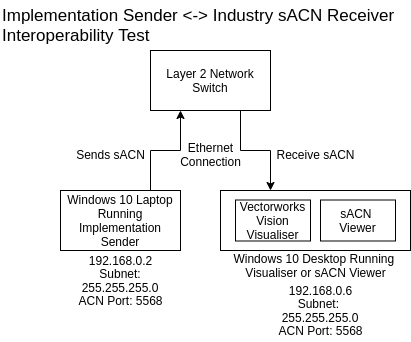
\includegraphics[width=\textwidth]{CS4099-Visualiser-setup.png}
	\caption{The set-up of the sender implementation interoperability test}
\end{figure}

\begin{figure}[H]
	\label{VIS_LX_PLOT}
	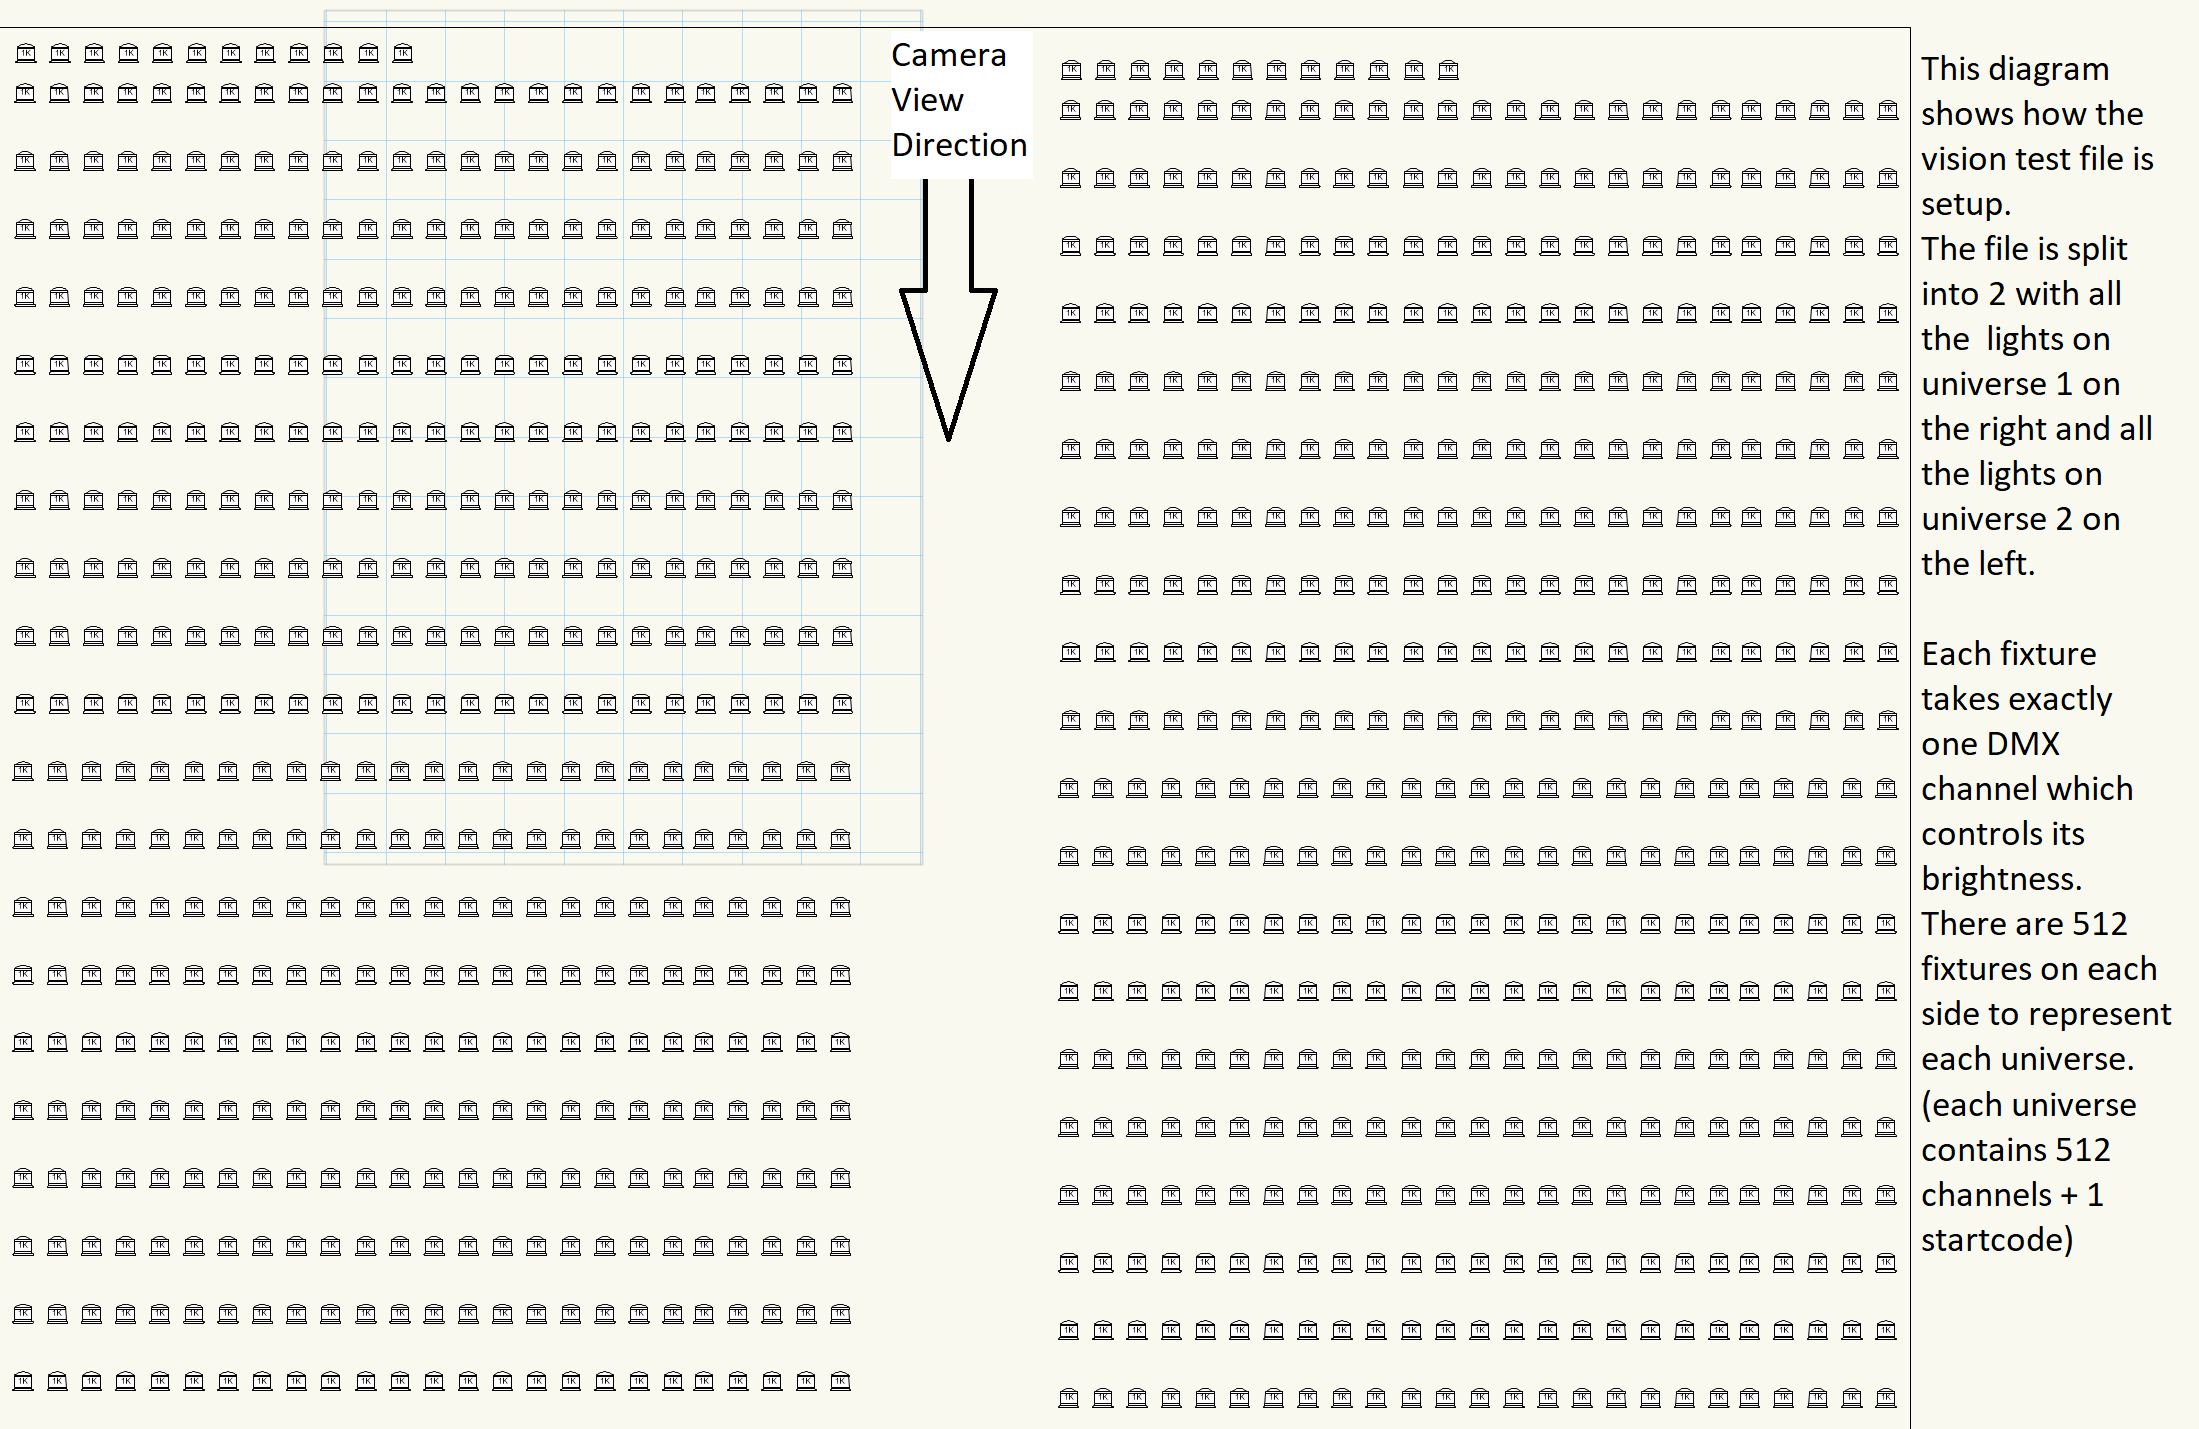
\includegraphics[width=\textwidth]{Vision-File-LX-Plot.png}
	\caption{The lighting plot of the lights used as part of the Vision Visualiser test scene}
\end{figure}

\subsubsection{Acceptance Testing}
Acceptance testing is the final stage of testing within the project and represents the transition from the testing phase to the deployment phase. For this test a similar setup is used to the external interoperability tests however this time rather than just the developer these tests were performed in the presence of an industry professional. This allows demonstrating that the program can actually be used for its intended purpose, it also allows the chance for people in industry (the targeted end users) to provide feedback or evaluation about the usefulness of the program and point out potential problems. \\

Two separate demonstrations are performed, first showing the functionality of the program as a sender with data sent from the implementation to the visualiser with the person seeing both the commands entered into the implementation sender and the results on the visualiser. The second demonstration shows the sACN source lighting board (Avolites Titan) sending to the receiver with the data received displayed on the screen in text format. \\

The industry professional for this test was the Technical Supervisor for the St Andrews Students Association. As a technician they work with lighting, sound and other entertainment systems daily and so they are ideally placed to demonstrate the implementation of this widely used lighting protocol to. The visualisation test provides significant value to the project as a professional working in the field will know how this fits into the real-world work flow of someone working in lighting and therefore that this is an actual representative usage of the protocol. The receiver output from the lighting board is also extremely valuable as the technician is able to observe that this is a real-world sACN source which is being used with the protocol and they can see that the data is being correctly sent by the board and received as expected.  \\

The test layout is shown in \ref{ACCEPTANCE_TEST_LAYOUT}, the plan for the demonstrations to run are detailed in the "CS4099 - Interoperability Testing" however during the actual test there is the possibility of questions which may lead the demonstration to change to show specific areas of the implementation. Once this test was complete the professional then agreed to write up a short email describing the test and their evaluation of the demonstration.\\ 

The lighting layout used for visualisation in this test is setup to be similar to the actual setup used in the students union thereby being a representative example of an actual industry use case. The layout of this setup with accompanying explanation is shown in figure \ref{ACCEPTANCE_TEST_LX_PLOT}. 

\begin{figure}[H]
	\label{ACCEPTANCE_TEST_LAYOUT}
	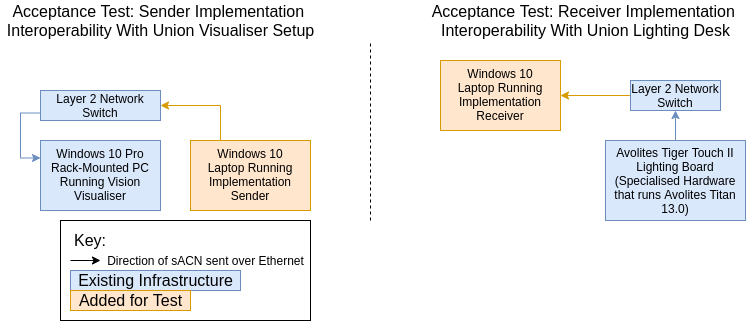
\includegraphics[width=\textwidth]{CS4099-Acceptance-Test-Layout.png}
	\caption{The layout of the acceptance test performed}
\end{figure}

\begin{figure}[H]
	\label{ACCEPTANCE_TEST_LX_PLOT}
	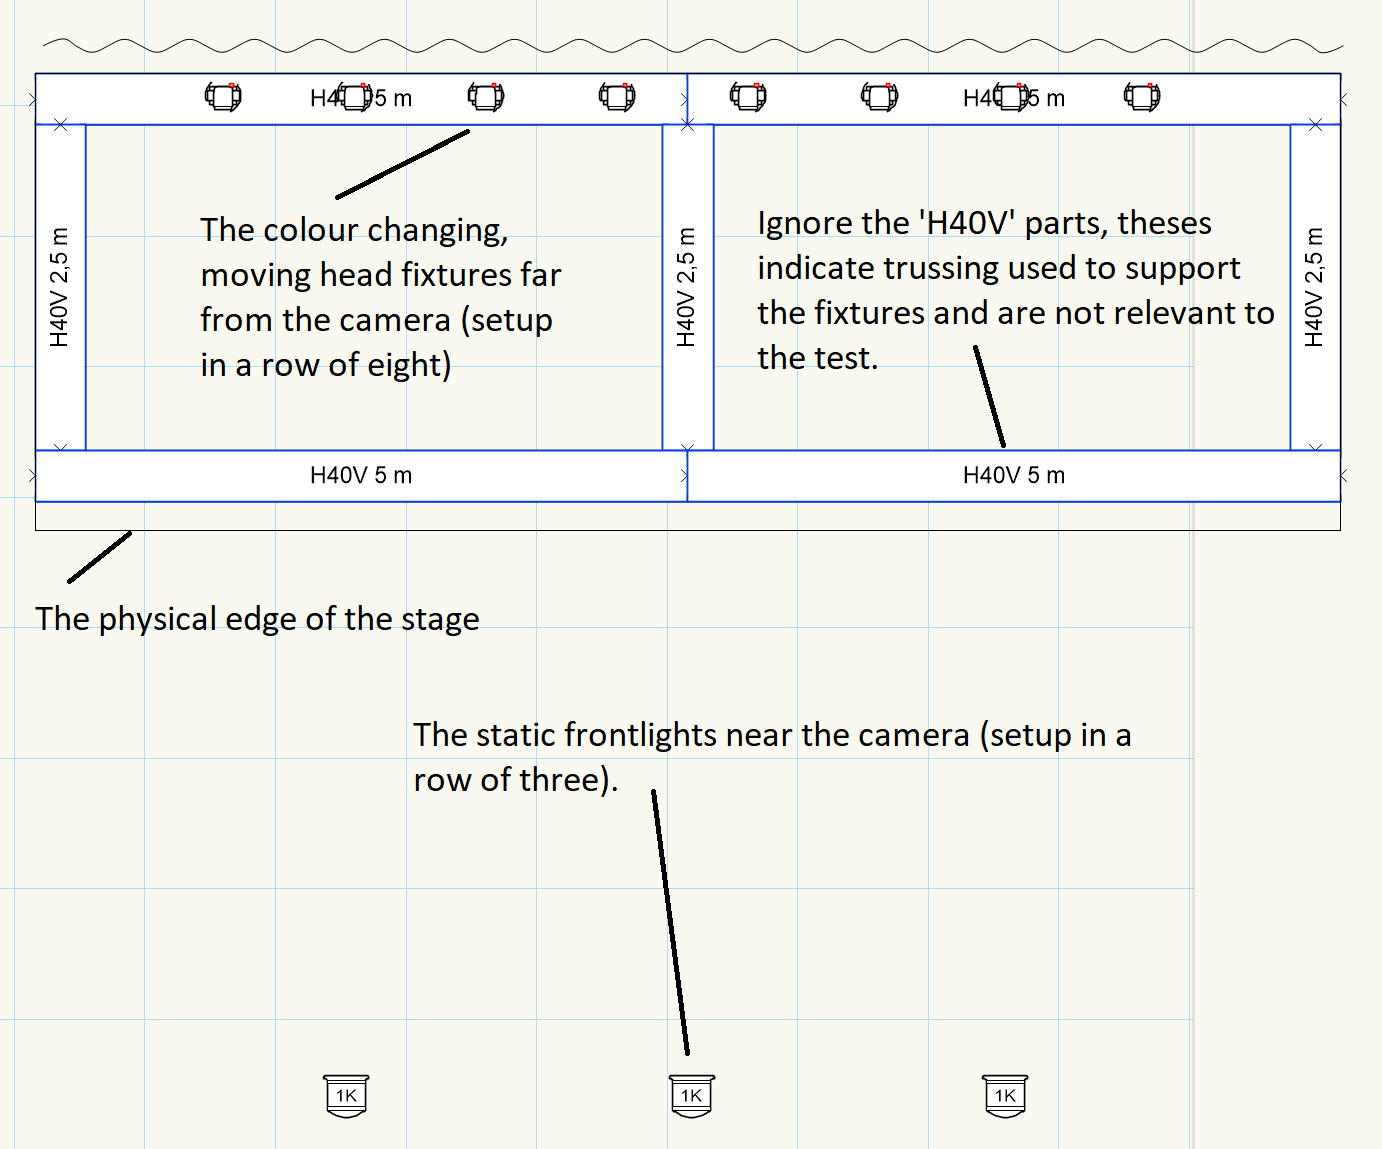
\includegraphics[width=\textwidth]{Union-Setup-Vision-File-LX-Plot.png}
	\caption{The lighting plot showing the locations and addresses of fixtures within the visualiser used as part of the acceptance test. This is based on the actual lighting layout used within the students association. Additional explanation has been added on top of the plan to describe what each part means.}
\end{figure}

\subsection{What Testing Shows}
The unit and integration tests in combination with the code-coverage show that the code works as expected but to show that the behaviour actually fits with the protocol specification compliance testing was performed. Ideally this would be done through an external compliance test suite however none exist public-ally for the protocol. Therefore a compliance suite was created, this was done by going through the protocol specification document \cite{ANSI_E1.31} and generating a list of required functionality for each section, unit and integration tests were then created so that each requirement was fulfilled. This systematic approach makes it much less likely that something will be missed and increases confidence that the implementation will be compliant with all aspects of the protocol. This table is included in the attached "Protocol Compliance Test Sheet.pdf" document coloured coded to show the results of the tests for each requirement. Further to this the interoperability tests also provide evidence that the implementation is compliant because the programs used have been shown to be compliant themselves so being interoperable through the protocol indicates the implementation is compliant. The acceptance test then provides evidence that the implementation can actually be used as expected. This testing therefore shows the progress from design to implementation through to a deployable compliant implementation.

\section{Evaluation and Critical Appraisal}
Evaluation and critical appraisal
You should evaluate your own work with respect to your original objectives. You should also critically evaluate your work with respect to related work done by others. You should compare and contrast the project to similar work in the public domain, for example as written about in published papers, or as distributed in software available to you.

There exists no fully-implemented public-ally available implementation of sACN in rust and the most complete version was used as the base of this project, this means that there is no direct comparison possible between this project and another however there do exist many implementations sACN in other languages so these can be used for comparison. \\


The decision not to pass up data packets awaiting synchronisation means that the packets must be temporarily stored within the receiver and this is done using a Vec data-structure which is a dynamically sized structure. This means that the memory allocated to the program will continue to increase as packets are received which can be problematic for embedded devices with limited memory capacity. To limit this problem the implementation relies on the limited number of possible universes in the protocol and only stores a single universe of data for each waiting universe. This limits the maximum required space for this storage to 31.3MB + overhead which is not a problem for any modern PC but is potentially a significant amount for an embedded device. This means that the library is at risk of running out of memory for some devices such as arduino \cite{ARDUINO} which are commonly used for creating simple DIY embedded systems. This is only a risk on systems which have a large number of universes being synchronised at once so the for majority of usage cases where most universes aren't synchronised and only a few are synchronised at any one time this isn't a problem. To avoid this problem on an embedded system it is therefore required to keep the number of universes being listened to 'low' (other universe packets are discarded) with 'low' decided by the resources available (based on benchmarks etc.).  
\[ 
\textit{max possible universes} \times \textit{universe capacity} = 63999 \times 513 B \approxeq 31.3 megabytes. 
\]

The library is based on the std-environment. This means the implementations utilises the standard rust crates to provide functionality such as hash-maps and threads. This decisions means that the produced binary is potentially bigger than it otherwise might be and isn't as tuned to the specific application from the perspective of performance. These costs come at an advantage however as re-using standard libraries means that the required features don't have to be re-implemented from scratch. This limits the testing required and reduces the chance of bugs as the existing implementations are already widely used and tested. It also reduces the development time required significantly which was vital to allow this project to be completed within the time-allowed. It would not have been possible to create the library within the given-time without utilising at least some existing libraries/implementations such as std.\\

The receiver uses a single threaded design with the timeout for all source+universe sequence numbers being checked when any sequence number is checked. As every source/uni combination is checked everytime a sequence number is checked this comes with a performance hit as they all must be visited each time. This is required because otherwise a source which has completely stopped transmitting on a universe and for which the termination packets are lost would never be removed from the sequence numbers and would take up space on the receiver continuously which is problematic for embedded devices. While not used within this implementation an alternative strategy could be to only check time-outs occasionally (say every 5 sequence number checks) or to have the timeout checks be done periodically based on a time interval. This would reduce the number of checks required and therefore theoretically increase performance at the cost of having dead-universe and source sequence numbers stored longer than is required.\\

	
The library is based on wrapping an underlying socket which is used to access the underlying transport UDP protocol. The library does not provide a way to change how this underlying mechanism works
-- More abstractions means a performance cost
-- The implementation has to be on the heap due to the rust system (in a dyn box) as the size isn't known at compile time (or does it -> sized trait?)
-- Using a swappable underlying abstraction allowed easier testing as a test sender and receiver could be created. These test implementations rather than actually sending were then used to log output and create input to the protocol. 
-- By using this abstraction and allowing a more modular design it makes later changes easier. This reduces the cost of making changes or bug fixes especially in the maintenance phase as changes to the underlying implementation don't effect the rest of the code base. This also allows the underlying protocol to change, similarly to how between ANSI E1.31-2016 and -2018 IPv6 was added it allows later versions to add support for other network or transport protocols. The abstraction also allows the user to add support for more platforms for example how in the implementation there are 2 versions of the network receiver one for Windows and one for Linux/Fedora. These different versions are required as different operating systems treat sockets differently as not all operating systems comply to standards such as POSIX. This is especially true with embedded devices which might have hardware specific mechanisms for sending/receiving due to limited resources.


-- Only supports Windows/Linux, outwith scope to supports more operating systems, no test devices.
-- Library doesn't aim to be fully compliant with every feature.

// Report note:
// One of the problems with the existing SACN sending is how it didn't treat the payload transparently because it 
// would add on the start code. As this is part of the DMX protocol and not the SACN protocol this was removed as it 
// violated the extends of SACN.
// Report: The first universe for the data to be synchronised across multiple universes is 
// used as the synchronisation universe by default. This is done as it means that the receiver should
// be listening for this universe. 

The PoisonError problem, rust is still developing and there isn't a standard error system, PoisonError cannot be used with other error types... 

// Report: Should start code be seperated out when receiving? Causes input and output to differ and is technically part of another protocol.
// - Decided it shouldn't be seperated.

/// For some tests to work multiple instances of the protocol must be on the same network with the same port for example to test multiple simultaneous receivers, this means multiple IP's are needed.
/// This is achieved by assigning multiple static IP's to the test machine and theses IP's are specified below.
/// Theses must be changed depending on the network that the test machine is on.

Couldn't show that the receiver worked with universe synchronisation or discovery. This is because the real-world sACN sender used (Avolites Titan) does not support it. Ideally another source would have been used however an initial inspection found none that did support it that could be used. If there had been time a test program could have been written using a library in another programming language and this used however there was insufficient time to learn, write and test an entirely new library in another language so that it could be used for this test.
 
\subsection{Extraneous Circumstances - COVID-19}
Unfortunately the acceptance test which was planned for sometime between the 14th and 29th of March based on when the technician was free was unable to take place. This is due to the outbreak of the COVID-19 virus which forced the students association to close and non-essential contact to be stopped before the demonstration could be conducted. It is predicted that based on the very similar integration tests passing as-well as the other testing that had the demonstration gone ahead the program would have worked as expected and the evaluation been positive. It is a shame that the test could not be conducted as comments could have led to recommended improvements for the project which would have ultimately resulted in a higher quality submission. An annotated video is included showing what one of the acceptance tests may have looked like although this video is performed on my own hardware rather than the students union equipment.\\

The COVID-19 also meant that I was unable to remain in St Andrews and continue to have access to the computing labs. This had a number of impacts. The first was the time lost due to the move and having to create a new setup for working at home. This environment was less than ideal and meant that some features which may have been possible had things continued as normal were not. The move also meant that I no longer had direct access to more than 1-2 machines. This means that tests like the ssh integration tests were much more difficult to create because they had to be done completely remotely from home SSH'd into labs. This lead to far fewer of these tests being created than would have been hoped. \\

\section{Conclusions}
Conclusions
You should summarise your project, emphasising your
key achievements and significant drawbacks to your
work, and discuss future directions your work could be
taken in.

-- Finish full compliance, performance analysis vs C, see how the library does and if worth using in actual devices. 

\section{Appendices}
The appendices to your report will normally be as follows.
Testing
summary
This should describe the steps taken to debug, test,
verify or otherwise confirm the correctness of the
various modules and their combination.

\section{User Manual}
User manual Instructions on installing, executing and using the
system where appropriate.\\

The core part of this project was the sACN library created. This library is packaged as a rust cargo crate and therefore can be imported using a local import as demonstrated in the 'demo\_src' and 'demo\_rcv' programs. After this project is complete the project will hopefully be uploaded to the public rust cargo repository which would allow much easier installation through the 'cargo install' command.\\

Usage of the library is described in the generated rust-doc documentation. Once the project is complete this would also be bundled with the library in the public cargo repo to allow easier access however as that cannot be done until after this project is marked the documentation is included in the sacn subfolder of the doc folder. Within this folder the documentation can be opened as a web-page by opening the index.html file. This documentation contains details of the functionality of public and private functions as-well as the possible returned errors, examples of the code in usage and also includes the 'demo\_src' and 'demo\_rcv' crates.\\

The details of how to use the program are described in the usage.pdf file.

\section{Other Appendices}
Other
appendices
If appropriate, you may include other material in
appendices which are not suitable for inclusion in the
main body of your report, such as the ethical approval
document.
You should not include software listings in your project report, unless it is
appropriate to discuss small sections in the main body of your report. Instead,
you will submit via MMS your code and associated material such as JavaDoc
documentation and detailed UML diagrams

\begin{thebibliography}{9}
	\bibitem{ANSI_E1.17}
	ANSI E1.17 - 2015 Entertainment Technology?Architecture for Control Networks
	\bibitem{ORIGNIAL_IMPL}
	https://github.com/lschmierer/sacn (September 2019)
	\bibitem{ANSI_E1.31}
	ANSI E1.31 ? 2018 Entertainment Technology Lightweight streaming protocol for transport of DMX512 using ACN
	\bibitem{DMX_INFO}
	https://www.element14.com/community/groups/open-source-hardware/blog/2017/08/24/dmx-explained-dmx512-and-rs-485-protocol-detail-for-lighting-applications (17/09/2019)
	\bibitem{C_IMPL}
	https://github.com/hhromic/libe131 (17/09/2019)
	\bibitem{RUST_LANG}
	https://www.rust-lang.org/ (17/09/2019)
	\bibitem{ARTNET}
	http://artisticlicence.com/WebSiteMaster/User\%20Guides/art-net.pdf (17/09/2019)
	\bibitem{ORIGINAL_IMPL_RUST_DOC}
	https://docs.rs/sacn/0.4.4/sacn/index.html
	(26/01/2020)
	\bibitem{C++_IMPL}
	https://github.com/hhromic/libe131
	(26/01/2020)
	\bibitem{ANSI_E1.31_2009}
	https://tsp.esta.org/tsp/documents/docs/E1-31\_2009.pdf
	(26/01/2020)
	\bibitem{ANSI_E1.31_2016}
	https://tsp.esta.org/tsp/documents/docs/E1-31-2016.pdf
	(26/01/2020)
	\bibitem{WHAT_COMES_AFTER_SACN}
	http://www.rdmprotocol.org/files/What\_Comes\_After\_Streaming\_DMX\_over\_ACN\_\%20\%284\%29.pdf (26/01/2020)
	\bibitem{ANSI_E1.33_2019}
	RDM-NET
	\bibitem{ANSI_E1.33_IMPL}
	https://github.com/ETCLabs/RDMnet (26/01/2020)
	\bibitem{ANSI_E1.20_2010}
	RDM
	\bibitem{ETC}
	https://www.etcconnect.com/About/ (26/01/2020)
	\bibitem{RUST_C_COMPARISON}
	https://benchmarksgame-team.pages.debian.net/benchmarksgame/fastest/rust.html (28/01/2020)
	\bibitem{WHY_LEARN_RUST}
	https://www.techrepublic.com/article/rust-programming-language-seven-reasons-why-you-should-learn-it-in-2019/
	\bibitem{waterfall-diagram}
	https://www.tutorialspoint.com/sdlc/sdlc\_waterfall\_model.htm (01/01/2020)
	\bibitem{ETHERNET_MTU}
	https://tools.ietf.org/html/rfc894 (10/03/2020)
	\bibitem{NO_STD_LIB}
	https://doc.rust-lang.org/1.7.0/book/no-stdlib.html (11/03/2020)
	\bibitem{ARDUINO}
	https://www.arduino.cc/en/tutorial/memory (11/03/2020)
	\bibitem{RUST_TRY}
	https://doc.rust-lang.org/std/macro.try.html (12/03/2020)
	\bibitem{ERROR_CHAIN}
	https://github.com/rust-lang-nursery/error-chain (12/03/2020)
	\bibitem{WIRESHARK}
	https://www.wireshark.org/ (12/03/2020)		
	\bibitem{SACN_VIEW}
	https://sacnview.org/ (12/03/2020)
	\bibitem{SACN_VIEW_DOC}
	https://sacnview.org/documentation.html (12/03/2020)
	\bibitem{VISION}
	https://www.vectorworks.net/en-GB/vision (12/03/2020)
	\bibitem{AVO_TITAN_MOBILE}
	https://www.avolites.com/product/titan-mobile/ (12/03/2020)
	\bibitem{NET_STACK_IMAGE}
	https://www.dcs.bbk.ac.uk/~ptw/teaching/IWT/transport-layer/notes.html (13/03/2020)
	\bibitem{IETF_RFC_5771}
	https://tools.ietf.org/html/rfc5771
	\bibitem{IETF_RFC_2365}
	https://tools.ietf.org/html/rfc2365
	\bibitem{IETF_RFC_4291}
	https://tools.ietf.org/html/rfc4291
	\bibitem{UNIT_TESTING}
	http://softwaretestingfundamentals.com/unit-testing/ (06/04/2020)
	\bibitem{GRCOV}
	https://github.com/mozilla/grcov (06/04/2020)
	\bibitem{CODE_COVERAGE}
	https://martinfowler.com/bliki/TestCoverage.html
	\bibitem{RUST_AFL_FUZZ}
	https://github.com/rust-fuzz/afl.rs (08/04/2020)
	\bibitem{RUST_AFL_FUZZ_DOC}
	https://rust-fuzz.github.io/book/afl.html (08/04/2020)
	\bibitem{WIRESHARK_EXPORT_RAW}
	https://www.wireshark.org/docs/wsug\_html\_chunked/ChIOExportSection.html (08/04/2020)
\end{thebibliography}

\end{document}